\input{preamble.tex}

\begin{document}

\thispagestyle{fancy}

\begin{center}
\LARGE\scshape Categorical Representation Theory\noindent\\[-\linespacing]
\rule{0.75\linewidth}{1pt}
\end{center}
\noindent\\[-0.75\linespacing]

\ruledsection{Prologue}{1}
\noindent\\ Before we get into representation theory, let's {\em very} briefly review some basic definitions from higher category theory. We will follow \cite{Mal18} and \cite[\S 9]{Str95} as our main references.\\

\noindent\begin{definition}\textnormal{(Bicategory).} A {\em bicategory} $\mathscr{C}$ consists of
\begin{enumerate}[label=$\bullet$, leftmargin=4\parindent]
\item a class $\obset(\mathscr{C})$ of {\em objects} (or {\em $0$-cells});
\item for each pair of objects $\textobj{i}, \textobj{j} \in \obset(\mathscr{C})$, a {\em Hom-category} $\mathscr{C}(\textobj{i}, \textobj{j})$ whose objects are called {\em $1$-morphisms} (or {\em $1$-cells}), whose morphisms are called {\em $2$-morphisms} (or {\em $2$-cells}) and where composition of $2$-morphisms is known as {\em vertical composition} and denoted $\circ_v$;
\item for each triple of objects $\textobj{i}, \textobj{j}, \textobj{k} \in \obset(\mathscr{C})$, a functor $\circ_h : \mathscr{C}(\textobj{j}, \textobj{k}) \times \mathscr{C}(\textobj{i}, \textobj{j}) \to \mathscr{C}(\textobj{i}, \textobj{k})$ known as {\em horizontal composition};
\item for each object $\textobj{i} \in \obset(\mathscr{C})$, a distinguished $1$-morphism $\textnormal{id}_\textobj{i} \in \morset(\mathscr{C}(\textobj{i}, \textobj{i}))$ known as the {\em identity morphism} for $\textobj{i}$;
\item for each pair of objects $\textobj{i}, \textobj{j} \in \obset(\mathscr{C})$, natural isomorphisms $l$ and $r$ satisfying
\begin{align*}
\begin{split}
\begin{pmatrix}f \mapsto \textnormal{id}_\textobj{j} \circ_h f\\\alpha \mapsto \textnormal{id}_{\textnormal{id}_\textobj{j}} \circ_h \alpha\end{pmatrix} \xRightarrow{l} \begin{pmatrix}f \mapsto f\\\alpha \mapsto \alpha\end{pmatrix} \xLeftarrow{r} \begin{pmatrix}f \mapsto f \circ_h \textnormal{id}_\textobj{i}\\\alpha \mapsto \alpha \circ_h \textnormal{id}_{\textnormal{id}_\textobj{i}}\end{pmatrix}\!,
\end{split}
\end{align*}
known respectively as a {\em left} and {\em right unitor} (whose components $l_f$ and $r_f$ are $2$-morphisms);
\item for each quadruple of objects $\textobj{i}, \textobj{j}, \textobj{k}, \textobj{l} \in \obset(\mathscr{C})$, a natural isomorphism $a$ between the two horizontal composition functors $\mathscr{C}(\textobj{k}, \textobj{l}) \times \mathscr{C}(\textobj{j}, \textobj{k}) \times \mathscr{C}(\textobj{i}, \textobj{j}) \to \mathscr{C}(\textobj{i}, \textobj{l})$ given by
\begin{align*}
\begin{split}
\begin{pmatrix}h \times g \times f \mapsto (h \circ_h g) \circ_h f\\\gamma \times \beta \times \alpha \mapsto (\gamma \circ_h \beta) \circ_h \alpha\end{pmatrix} \xRightarrow{a} \begin{pmatrix}h \times g \times f \mapsto h \circ_h (g \circ_h f)\\\gamma \times \beta \times \alpha \mapsto \gamma \circ_h (\beta \circ_h \alpha)\end{pmatrix}\!,
\end{split}
\end{align*}
known as an {\em associator} (whose components $a_{h, g, f}$ are $2$-morphisms);
\end{enumerate}
\noindent such that the pentagon diagram
\begin{center}
\begin{tikzcd}
& ((k \circ_h h) \circ_h g) \circ_h f\arrow[dl, "a_{k, h, g} \circ_h \textnormal{id}_f"']\arrow[dr, "a_{k \circ_h h, g, f}"] &\\ %\arrow[dl, "a_{\textobj{j}, \textobj{k}, \textobj{l}, \textobj{m}} \circ_h \textnormal{id}_{\mathscr{C}(\textobj{i}, \textobj{j})}"']\arrow[dr, "a_{\textobj{i}, \textobj{j}, \textobj{k}, \textobj{m}}"]
(k \circ_h (h \circ_h g)) \circ_h f\arrow[d, "a_{k, h \circ_h g, f}"'] && (k \circ_h h) \circ_h (g \circ_h f)\arrow[d, "a_{k, h, g \circ_h f}"]\\ %\arrow[d, "a_{\textobj{i}, \textobj{j}, \textobj{l}, \textobj{m}}"'] && \arrow[d, "a_{\textobj{i}, \textobj{k}, \textobj{l}, \textobj{m}}"]
k \circ_h ((h \circ_h g) \circ_h f)\arrow[rr, "\textnormal{id}_k\circ_h a_{h, g, f}"'] && k \circ_h (h \circ_h (g \circ_h f)) %\arrow[rr, "\textnormal{id}_{\mathscr{C}(\textobj{l}, \textobj{m})}\circ_h a_{\textobj{i}, \textobj{j}, \textobj{k}, \textobj{l}}"']
\end{tikzcd}
\end{center}
\noindent and the triangle diagram
\begin{center}
\begin{tikzcd}
(g \circ_h \textnormal{id}_\textobj{j}) \circ_h f\arrow[rr, "a_{g, \textnormal{id}_\textobj{j}, f}"]\arrow[dr, "r_g \circ_h \textnormal{id}_f"'] && g \circ_h (\textnormal{id}_\textobj{j} \circ_h f)\arrow[dl, "\textnormal{id}_g\circ_h l_f"]\\ %(g \circ_h \textnormal{id}_\textobj{j}) \circ_h f\arrow[rr, "a_{\textobj{i}, \textobj{j}, \textobj{j}, \textobj{k}}"]\arrow[dr, "r_{\textobj{j}, \textobj{k}}\circ_h \textnormal{id}_{\mathscr{C}(\textobj{i}, \textobj{j})}"'] && g \circ_h (\textnormal{id}_\textobj{j} \circ_h f)\arrow[dl, "\textnormal{id}_{\mathscr{C}(\textobj{j}, \textobj{k})}\circ_h l_{\textobj{i}, \textobj{j}}"]\\
& g \circ_h f &
\end{tikzcd}
\end{center}
\noindent commute, for all $1$-morphisms $f \in \obset(\mathscr{C}(\textobj{i}, \textobj{j}))$, $g \in \obset(\mathscr{C}(\textobj{j}, \textobj{k}))$, $h \in \obset(\mathscr{C}(\textobj{k}, \textobj{l}))$, $k \in \obset(\mathscr{C}(\textobj{l}, \textobj{m}))$.
\end{definition}
\newpage

\noindent A $2$-category is a {\em strict} bicategory; that is, a bicategory whose unitors and associators are all identities. In this case the pentagon and triangle diagrams hold automatically. Observe that (strict) bicategories $\mathscr{C}$ with a single object $\bullet$ are in bijection with (strict) monoidal categories under taking the monoidal delooping; in particular, our monoidal category is nothing but the End-category $\mathscr{C}(\bullet, \bullet)$, where the monoidal product is given by horizontal composition.\\

\noindent We shall henceforth adopt the notation $\morset_\mathscr{C}^1(\textobj{i}, \textobj{j}) \coloneqq \obset(\mathscr{C}(\textobj{i}, \textobj{j}))$ and $\morset_\mathscr{C}^2(f, g) \coloneqq \morset_{\mathscr{C}(\textobj{i}, \textobj{j})}(f, g)$, for $\textobj{i}, \textobj{j} \in \obset(\mathscr{C})$ and $f, g \in \morset(\mathscr{C}(\textobj{i}, \textobj{j}))$. Unfortunately, we will frequently change our notation for $1$-morphisms and $2$-morphisms depending on what makes sense contextually. For instance, in light of the above remark, $1$-morphisms will often be objects of a monoidal category, whence we will write them as $X$, $Y$, $Z$ and so on; meanwhile, sometimes they will be realized as functors, in which case we will use $F$, $G$, $H$ and so on. The same goes for $2$-morphisms. We hope this will not cause any unnecessary confusion!\\

\noindent\begin{definition} \textnormal{(Pseudofunctor).} A {\em pseudofunctor} $\textnormal{F}$ between bicategories $\mathscr{C}$ and $\mathscr{D}$ consists of
\begin{enumerate}[label=$\bullet$, leftmargin=4\parindent]
\item a map $\textnormal{F} : \obset(\mathscr{C}) \to \obset(\mathscr{C})$;
\item for each pair of objects $\textobj{i}, \textobj{j} \in \obset(\mathscr{C})$, a functor $\textnormal{F} : \mathscr{C}(\textobj{i}, \textobj{j}) \to \mathscr{D}(\textnormal{F}(\textobj{i}), \textnormal{F}(\textobj{j}))$;
\item for each triple of objects $\textobj{i}, \textobj{j}, \textobj{k} \in \obset(\mathscr{C})$, a natural isomorphism $m$ between the two ``composition by $\textnormal{F}$'' functors $\mathscr{C}(\textobj{j}, \textobj{k}) \times \mathscr{C}(\textobj{i}, \textobj{j}) \to \mathscr{D}(\textnormal{F}(\textobj{i}), \textnormal{F}(\textobj{k}))$ given by
\begin{align*}
\begin{split}
\begin{pmatrix}g \times f \mapsto \textnormal{F}(g) \circ_h \textnormal{F}(f)\\\beta \times \alpha \mapsto \textnormal{F}(\beta) \circ_h \textnormal{F}(\alpha)\end{pmatrix} \xRightarrow{m} \begin{pmatrix}g \times f \mapsto \textnormal{F}(g \circ_h f)\\\beta \times \alpha \mapsto \textnormal{F}(\beta \circ_h \alpha)\end{pmatrix}\!, %\begin{pmatrix}g \times f \mapsto \textnormal{F}_{\textobj{j}, \textobj{k}}(g) \circ_h \textnormal{F}_{\textobj{i}, \textobj{j}}(f)\\\beta \times \alpha \mapsto \textnormal{F}_{\textobj{j}, \textobj{k}}(\beta) \circ_h \textnormal{F}_{\textobj{i}, \textobj{j}}(\alpha)\end{pmatrix} \xRightarrow{m_{\textobj{i}, \textobj{j}, \textobj{k}}} \begin{pmatrix}g \times f \mapsto \textnormal{F}_{\textobj{i}, \textobj{k}}(g \circ_h f)\\\beta \times \alpha \mapsto \textnormal{F}_{\textobj{i}, \textobj{k}}(\beta \circ_h \alpha)\end{pmatrix}\!;
\end{split}
\end{align*}
whose components $m_{g, f}$ are $2$-morphisms;
\item for each object $\textobj{i} \in \obset(\mathscr{C})$, an isomorphism $i : \textnormal{id}_{\textnormal{F}(\textobj{i})} \to \textnormal{F}(\textnormal{id}_\textobj{i})$ in $\morset(\mathscr{D}(\textnormal{F}(\textobj{i}), \textnormal{F}(\textobj{i})))$;
\end{enumerate}
\noindent such that the hexagon diagram
\begin{center}
\begin{tikzcd}
& (\textnormal{F}(h) \circ_h \textnormal{F}(g)) \circ_h \textnormal{F}(f)\arrow[dl, "m_{h, g} \circ_h \textnormal{id}_{\textnormal{F}(f)}"']\arrow[dr, "a_{\textnormal{F}(h), \textnormal{F}(g), \textnormal{F}(f)}"] & \\ % & (\textnormal{F}_{\textobj{k}, \textobj{l}}(h) \circ_h \textnormal{F}_{\textobj{j}, \textobj{k}}(g)) \circ_h \textnormal{F}_{\textobj{i}, \textobj{j}}(f)\arrow[dl, "m_{\textobj{j}, \textobj{k}, \textobj{l}} \circ_h \textnormal{id}_{\textnormal{F}(f)}"' {yshift = 1ex}]\arrow[dr, "a_{\textnormal{F}(\textobj{i}), \textnormal{F}(\textobj{j}), \textnormal{F}(\textobj{k}), \textnormal{F}(\textobj{l})}" {yshift = 1ex}] & \\
\textnormal{F}(h \circ_h g) \circ_h \textnormal{F}(f)\arrow[d, "m_{h \circ_h g, f}"'] && \textnormal{F}(h) \circ_h (\textnormal{F}(g) \circ_h \textnormal{F}(f))\arrow[d, "\textnormal{id}_{\textnormal{F}(h)} \circ_h m_{g, f}"]\\ %\textnormal{F}_{\textobj{j}, \textobj{l}}(h \circ_h g) \circ_h \textnormal{F}_{\textobj{i}, \textobj{j}}(f)\arrow[d, "m_{\textobj{i}, \textobj{j}, \textobj{l}}"'] && \textnormal{F}_{\textobj{k}, \textobj{l}}(h) \circ_h (\textnormal{F}_{\textobj{j}, \textobj{k}}(g) \circ_h \textnormal{F}_{\textobj{i}, \textobj{j}}(f))\arrow[d, "\textnormal{id}_{\textnormal{F}(h)} \circ_h m_{\textobj{i}, \textobj{j}, \textobj{k}}"]\\
\textnormal{F}((h \circ_h g) \circ_h f)\arrow[dr, "\textnormal{F}(a_{h, g, f})"'] && \textnormal{F}(h) \circ_h \textnormal{F}(g \circ_h f)\arrow[dl, "m_{h, g \circ_h f}"]\\ %\textnormal{F}_{\textobj{i}, \textobj{l}}((h \circ_h g) \circ_h f)\arrow[dr, "\textnormal{F}(a_{\textobj{i}, \textobj{j}, \textobj{k}, \textobj{l}})"'] && \textnormal{F}_{\textobj{k}, \textobj{l}}(h) \circ_h \textnormal{F}_{\textobj{i}, \textobj{k}}(g \circ_h f)\arrow[dl, "m_{\textobj{i}, \textobj{k}, \textobj{l}}"]\\
& \textnormal{F}(h \circ_h (g \circ_h f)) & % & \textnormal{F}_{\textobj{i}, \textobj{l}}(h \circ_h (g \circ_h f)) &
\end{tikzcd}
\end{center}
\noindent and the squares
\begin{center}
\begin{tikzcd}
%\textnormal{F}(g) \circ_h \textnormal{id}_{\textnormal{F}(\textobj{j})}\arrow[d, "r_{\textnormal{F}(g)}"']\arrow[r, "\textnormal{id}_{\textnormal{F}(g)} \circ_h i" {yshift = 1ex}] & \textnormal{F}(g) \circ_h \textnormal{F}(\textnormal{id}_\textobj{j})\arrow[d, "m_{g, \textnormal{id}_\textobj{j}}"]\\
%\textnormal{F}(g) & \textnormal{F}(g \circ_h \textnormal{id}_\textobj{j})\arrow[l, "\textnormal{F}(r_g)" {yshift = -1ex}]
\textnormal{id}_{\textnormal{F}(\textobj{j})} \circ_h \textnormal{F}(f)\arrow[d, "i \circ_h \textnormal{id}_{\textnormal{F}(f)}"']\arrow[r, "l_{\textnormal{F}(f)}"] & \textnormal{F}(f)\\
\textnormal{F}(\textnormal{id}_\textobj{j}) \circ_h \textnormal{F}(f)\arrow[r, "m_{\textnormal{id}_\textobj{j}, f}"' {yshift = -0.75ex}] & \textnormal{F}(\textnormal{id}_\textobj{j} \circ_h f)\arrow[u, "\textnormal{F}(l_f)"']
\end{tikzcd}\quad and \quad\begin{tikzcd}
%\textnormal{F}(\textnormal{id}_\textobj{j}) \circ_h \textnormal{F}(f)\arrow[d, "m_{\textnormal{id}_\textobj{j}, f}"'] & \textnormal{id}_{\textnormal{F}(\textobj{j})} \circ_h \textnormal{F}(f)\arrow[d, "l_{\textnormal{F}(f)}"]\arrow[l, "i \circ_h \textnormal{id}_{\textnormal{F}(f)}"' {yshift = 1ex}]\\
%\textnormal{F}(\textnormal{id}_\textobj{j} \circ_h f)\arrow[r, "\textnormal{F}(l_f)"' {yshift = -1ex}] & \textnormal{F}(f)
\textnormal{F}(f) \circ_h \textnormal{id}_{\textnormal{F}(\textobj{i})}\arrow[d, "\textnormal{id}_{\textnormal{F}(f)} \circ_h i"']\arrow[r, "r_{\textnormal{F}(f)}"] & \textnormal{F}(f)\\
\textnormal{F}(f) \circ_h \textnormal{F}(\textnormal{id}_\textobj{i})\arrow[r, "m_{f, \textnormal{id}_\textobj{i}}"' {yshift = -0.75ex}] & \textnormal{F}(f \circ_h \textnormal{id}_\textobj{i})\arrow[u, "\textnormal{F}(r_f)"']
\end{tikzcd}
\end{center}
\noindent commute, for all $1$-morphisms $f \in \obset(\mathscr{C}(\textobj{i}, \textobj{j}))$, $g \in \obset(\mathscr{C}(\textobj{j}, \textobj{k}))$, $h \in \obset(\mathscr{C}(\textobj{k}, \textobj{l}))$.
\end{definition}

\noindent As before, a $2$-functor is a pseudofunctor where $m$ and $i$ are identity. In the same way that bicategories generalize monoidal categories, pseudofunctors generalize strong monoidal functors, preserving both vertical composition (strictly) and horizontal composition (up to isomorphism).\\

\noindent\begin{definition}\textnormal{(Pseudonatural Transformation).} A {\em pseudonatural transformation} $\Phi$ between\linebreak pseudofunctors $\textnormal{F}$ to $\textnormal{G}$ consists of
\begin{enumerate}[label=$\bullet$, leftmargin=4\parindent]
\item for each object $\textobj{i} \in \obset(\mathscr{C})$, a $1$-morphism $\Phi_\textobj{i} \in \obset(\mathscr{D}(\textnormal{F}(\textobj{i}), \textnormal{G}(\textobj{i})))$;
\item for each $1$-morphism $f \in \obset(\mathscr{C}(\textobj{i}, \textobj{j}))$, a $2$-morphism $\Phi_f : \Phi_\textobj{j} \circ_h \textnormal{F}(f) \to \textnormal{G}(f) \circ_h \Phi_\textobj{i}$ in $\morset(\mathscr{D}(\textnormal{F}(\textobj{i}), \textnormal{G}(\textobj{j})))$;
\end{enumerate}
\noindent such that
\begin{enumerate}[label=$\bullet$, leftmargin=4\parindent]
\item for each $2$-morphism $\alpha : f \to g$ in $\morset(\mathscr{C}(\textobj{i}, \textobj{j}))$, the square
\begin{center}
\begin{tikzcd}
\Phi_\textobj{j} \circ_h \textnormal{F}(f)\arrow[d, "\Phi_f"']\arrow[r, "\textnormal{id}_{\Phi_\textobj{j}} \circ_h \textnormal{F}(\alpha)" {yshift = 0.75ex}] & \Phi_\textobj{j} \circ_h \textnormal{F}(g)\arrow[d, "\Phi_g"]\\
\textnormal{G}(f) \circ_h \Phi_\textobj{i}\arrow[r, "\textnormal{G}(\alpha) \circ_h \textnormal{id}_{\Phi_\textobj{i}}"' {yshift = -0.75ex}] & \textnormal{G}(g) \circ_h \Phi_\textobj{i}
\end{tikzcd}
\end{center}
commutes (that is, the $2$-morphisms $\Phi_f$ are the components of a natural transformation);
\item for each pair of $1$-morphisms $f \in \obset(\mathscr{C}(\textobj{i}, \textobj{j}))$, $g \in \obset(\mathscr{C}(\textobj{j}, \textobj{k}))$, the octagon diagram
\begin{center}
\begin{tikzcd}
&[-5em] (\Phi_\textobj{k} \circ_h \textnormal{F}(g)) \circ_h \textnormal{F}(f)\arrow[dl, "\Phi_g \circ_h \textnormal{id}_{\textnormal{F}(f)}"']\arrow[r, "a_{\Phi_\textobj{k}, \textnormal{F}(g), \textnormal{F}(f)}" {yshift = 0.75ex}] & \Phi_\textobj{k} \circ_h (\textnormal{F}(g) \circ_h \textnormal{F}(f))\arrow[dr, "\textnormal{id}_{\Phi_\textobj{k}} \circ_h m_{g, f}"] &[-4em] \\
(\textnormal{G}(g) \circ_h \Phi_\textobj{j}) \circ_h \textnormal{F}(f)\arrow[d, "a_{\textnormal{G}(g), \Phi_\textobj{j}, \textnormal{F}(f)}"'] &&& \Phi_\textobj{k} \circ_h \textnormal{F}(g \circ_h f)\arrow[d, "\Phi_{g \circ_h f}"]\\
\textnormal{G}(g) \circ_h (\Phi_\textobj{j} \circ_h \textnormal{F}(f))\arrow[dr, "\textnormal{id}_{\textnormal{G}(g)} \circ_h \Phi_f"'] &&& \textnormal{G}(g \circ_h f) \circ_h \Phi_\textobj{i}\\
& \textnormal{G}(g) \circ_h (\textnormal{G}(f) \circ_h \Phi_\textobj{i}) & (\textnormal{G}(g) \circ_h \textnormal{G}(f)) \circ_h \Phi_\textobj{i}\arrow[l, "a_{\textnormal{G}(g), \textnormal{G}(f), \Phi_\textobj{i}}" {yshift = -1ex}]\arrow[ur, "m_{g, f} \circ_h \textnormal{id}_{ \Phi_\textobj{i}}"'] &
\end{tikzcd}
\end{center}
commutes;
\item for each object $\textobj{i} \in \obset(\mathscr{C})$, the pentagon diagram
\begin{center}
\begin{tikzcd}
\Phi_\textobj{i} \circ_h \textnormal{id}_{\textnormal{F}(\textobj{i})}\arrow[d, "\textnormal{id}_{\Phi_\textobj{i}} \circ_h i"']\arrow[r, "r_{\Phi_\textobj{i}}"] & \Phi_\textobj{i} & \textnormal{id}_{\textnormal{G}(\textobj{i})} \circ_h \Phi_\textobj{i}\arrow[l, "l_{\Phi_\textobj{i}}"']\arrow[d, "i \circ_h \textnormal{id}_{\Phi_\textobj{i}}"]\\
\Phi_\textobj{i} \circ_h \textnormal{F}(\textnormal{id}_\textobj{i})\arrow[rr, "\Phi_{\textnormal{id}_\textobj{i}}"'] && \textnormal{G}(\textnormal{id}_\textobj{i}) \circ_h \Phi_\textobj{i}
\end{tikzcd}
\end{center}
commutes.
\end{enumerate}
\noindent If each $\Phi_f$ is invertible (they form a natural isomorphism), we call $\Phi$ a {\em pseudonatural isomorphism}.\\
\end{definition}

\noindent We say that two bicategories are {\em biequivalent} if there exists an invertible pseudofunctor between them. For the sections that follow, we will assume that all categories are essentially small, that all bicategories are essentially small and that all fields are algebraically closed.
\newpage

%\noindent\textcolor{red}{Throughout these notes, we will often talk about both weak and strict $2$-categories. We will use ``bicategory'' to mean a weak $2$-category, which roughly consists of a class of objects, a class of $1$-morphisms between objects and a class of $2$-morphisms between $1$-morphisms, together with unitors, associators and a notion of horizontal composition. Meanwhile, a ``$2$-category'' will be taken to mean a strict $2$-category, which is roughly a bicategory whose unitors and associators are equalities rather than mere natural transformations. Note that there is a bijection between one-object bicategories (respectively, $2$-categories) and monoidal (respectively, strict monoidal) categories. We will also assume that $\mathbbm{k}$ is an algebraically closed field.}\\

%\noindent\textcolor{red}{Should be more precise and put basic module category (including 7.1.3 of EGNO) and higher category theoretic definitions here, as well as assumptions like bicategories being essentially small and fields being algebraically closed. We should also mention conventions, like pseudofunctors being what \cite{Lei98} calls homomorphisms (roughly associates with each pair of Hom-categories a functor), natural transformations between pseudofunctors being strong transformations (roughly associates with each pair of functors a natural transformation), etc. Finally, we should mention notation, like $\simeq$ being used for equivalences of categories and $\cong$ being used for isomorphisms.}\\

\noindent\textcolor{red}{Note that given a bicategory $\mathscr{C}$ and objects $X, Y \in \obset(\mathscr{C})$, we have that $\mathscr{C}(X, Y)$ is a\linebreak $(\mathscr{C}(X, X), \mathscr{C}(Y, Y))$-bimodule category. Check bicategory of bifinite bimodules as in \cite{DGG14}.}\\

\noindent\textcolor{red}{\underline{Examples of bicategories.}}\\

\noindent\textcolor{red}{Given an algebra (or more generally a ring), one can build a $2$-category whose objects are algebras, $1$-morphisms are modules $(A, B)$-bimodules and $2$-morphisms are bimodule maps. In subfactor theory, we do this for a unital inclusion $N \subseteq M$ of type II$_1$ subfactors; we set $\obset(\mathscr{C}) \coloneqq \{M, N\}$ and $\mathscr{C}(X, Y) \coloneqq \textsf{Bimod}(X, Y)$ (``bimodule summands of basic constructions'' / bifinite $(X, Y)$-bimodules). This produces a $2$-category.}\\

\noindent\textcolor{red}{Given a shaded planar algebra $P$, take $\obset(\mathscr{C}) \coloneqq \{-, +\}$ and let $\mathscr{C}(\varepsilon, \eta) \coloneqq \textsf{Rect}_P(\varepsilon, \eta)$ be the subcategory of the rectangular category consisting of those morphisms whose domain shading is $\varepsilon$ and whose codomain shading is $\eta$, with composition running from bottom to top. In other words,
\begin{align*}
\begin{split}
\morset_\mathscr{C}^1(\varepsilon, \eta) \coloneqq \{2k : \text{$k \in \mathbb{N}$ is even if $\varepsilon = \eta$ and odd otherwise}\}
\end{split}
\end{align*}
\noindent and $\morset_\mathscr{C}^2(m, n) \coloneqq P_{m+n, \varepsilon}$, for $m, n \in \morset_\mathscr{C}^1(\varepsilon, \eta)$ (\cite{DGG14}). This gives a $\mathbb{C}$-linear (but unfortunately not additive) $2$-category. Look into ``The Temperley--Lieb algebra at roots of unity''.}\\

%this construction along with the above one gives a correspondence between unimodular bimodule planar algebras and finite index subfactors of type II$_1$ (I think? maybe only the reverse direction gives us this).

%\noindent\textcolor{red}{Given a shaded planar algebra $P$, take $\obset(\mathscr{C}) \coloneqq \{-, +\}$, let $\morset_{C}^1(X, Y)$ be the set of projections ($\pi = \pi^2 = \pi^*$) that lie in some $P_{2n, X}$, where $n$ is even if $Y = X$ and odd otherwise, and let $\morset_{C}^2(\pi_1, \pi_2)$ be the set of spaces of the form $\pi_2 \circ P_{m+n} \circ \pi_1$ for $\pi_1 \in P_{m, X}$ and $\pi_2 \in P_{n, Y}$ (https://arxiv.org/abs/0808.0764, pp.19-20).}\\

\noindent\textcolor{red}{Explicit example of multifinitary bicategory: group planar algebra? Maybe we can generalize it, see\\ https://scholars.unh.edu/cgi/viewcontent.cgi?article=1338\&context=dissertation.}\newpage

\ruledsection{Finitary Birepresentation Theory}{2}
\noindent\begin{definition}\textnormal{(Idempotent Complete).} Let $\mathcal{C}$ be a category. An {\em idempotent} is an endomorphism $p : A \to A$ in $\mathcal{C}$ such that $p \circ p = p$. An idempotent is said to {\em split} if there is an object $B$ and morphisms $\pi : A \to B$, $\iota : B \to A$ in $\mathcal{C}$ such that $p = \iota \circ \pi$ and $\textnormal{id}_B = \pi \circ \iota$. A category is said to be {\em idempotent complete} (or {\em idempotent split}) if every idempotent splits.\\
\end{definition}

\noindent Note that the condition $\textnormal{id}_B = \pi \circ \iota$ implies that $\pi$ is an epimorphism and $\iota$ is a monomorphism. To see why, suppose we have morphisms $h, k : B \to C$ with $h \circ \pi = k \circ \pi$. Then $h = h \circ \pi \circ \iota = k \circ \pi \circ \iota = k$, whence $\pi$ is an epimorphism. Similarly, given morphisms $h, k : C \to B$ with $\iota \circ h = \iota \circ k$, we have that $h = \pi \circ \iota \circ h = \pi \circ \iota \circ k = k$, whence $\iota$ is a monomorphism. Thus, because $\iota$ is a monomorphism, $B$ is by definition a subobject of $A$. In other words, a category being idempotent complete means that every idempotent $p : A \to A$ can be seen as a projection onto some subobject $B$ followed by an inclusion back into $A$. Moreover, in the additive setting we have the following result.\\

\noindent\begin{proposition} An idempotent $p : A \to A$ belonging to a preadditive category splits if and only if $A = \textnormal{Im}(p) \oplus \textnormal{Ker}(p)$.\\
\end{proposition}

\noindent\begin{proof} Suppose $p : A \to A$ is an idempotent that splits. Then by definition we have a subobject $I$ of $A$ together with an epimorphism $\pi_I : A \to I$ and a monomorphism $\iota_I : I \to A$ satisfying $p = \iota_I \circ \pi_I$ and $\textnormal{id}_{I} = \pi_I \circ \iota_I$. Moreover, because $\textnormal{id}_A - p$ is also idempotent, there similarly exists a subobject $K$ of $A$ together with an epimorphism $\pi_K : A \to K$ and a monomorphism $\iota_K : K \to A$ satisfying $\textnormal{id}_A - p = \iota_K \circ \pi_K$ and $\textnormal{id}_{K} = \pi_K \circ \iota_K$. Because $\textnormal{id}_A = \iota_I \circ \pi_I + \iota_K \circ \pi_K$, we have the biproduct diagram
\begin{center}
\begin{tikzcd}
I\arrow[r, shift right, "\iota_I"'] & A\arrow[l, shift right, "\pi_I"']\arrow[r, shift left, "\pi_K"] & K\arrow[l, shift left, "\iota_K"].
\end{tikzcd}
\end{center}
\noindent By \cite[Theorem VIII.2.2]{Mac13}, it follows that $A = I \oplus K$. We claim now that $\textnormal{Im}(p) = I$; we shall prove this by showing that $p$ admits the canonical decomposition
\begin{center}
\begin{tikzcd}
K\arrow[r, "\iota_K"] & A\arrow[r, "\pi_I"] & I\arrow[r, "\iota_I"] & A\arrow[r, "\pi_K"] & K.
\end{tikzcd}
\end{center}
\noindent In particular, we claim that $\textnormal{Ker}(p) = (K, \iota_K)$, that $\textnormal{Coker}(p) = (K, \pi_K)$, that $\textnormal{Coker}(\iota_K) = (I, \pi_I)$ and that $\textnormal{Ker}(\pi_K) = (I, \iota_I)$. We show that the first two hold and remark that showing the remaining two is essentially the same. First, observe that
\begin{align*}
\begin{split}
p \circ \iota_K = \iota_I \circ \pi_I \circ \iota_K = (\textnormal{id}_A - \iota_K \circ \pi_K) \circ \iota_K = \iota_K - \iota_K \circ \pi_K \circ \iota_K = \iota_K - \iota_K = 0.
\end{split}
\end{align*}
\noindent Moreover, given an object $K'$ together with a morphism $k' : K' \to A$ for which $p \circ k' = 0$, we see that by taking $\ell \coloneqq \pi_K \circ k'$, we have that
\begin{align*}
\begin{split}
\iota_K \circ \ell = \iota_K \circ \pi_K \circ k' = (\textnormal{id}_A - p) \circ k' = k'.
\end{split}
\end{align*}
\noindent Thus $\textnormal{Ker}(p) = (K, \iota_K)$. As for $\textnormal{Coker}(p)$, we observe that
\begin{align*}
\begin{split}
\pi_K \circ p = \pi_K \circ \iota_I \circ \pi_I = \pi_K \circ (\textnormal{id}_A - \iota_K \circ \pi_K) = \pi_K - \pi_K \circ \iota_K \circ \pi_K = \pi_K - \pi_K = 0,
\end{split}
\end{align*}
\noindent and that for any object $C'$ together with a morphism $c' : A \to C'$ for which $c' \circ p = 0$, taking $\ell \coloneqq c' \circ \iota_K$ gives us
\begin{align*}
\begin{split}
\ell \circ \pi_K = c' \circ \iota_K \circ \pi_K = c' \circ (\textnormal{id}_A - p) = c'.
\end{split}
\end{align*}
\noindent That $\textnormal{Coker}(\iota_K) = (I, \pi_I)$ and $\textnormal{Ker}(\pi_K) = (I, \iota_I)$ follow similarly, whence $A = \textnormal{Im}(p) \oplus \textnormal{Ker}(p)$.\newpage%\\[-1.5\baselineskip]
%\begin{center}
%\rule{0.5\linewidth}{1pt}
%\end{center}
%\noindent\\[-\baselineskip]
\noindent Conversely, suppose that $p : A \to A$ is an idempotent for which $A = \textnormal{Im}(p) \oplus \textnormal{Ker}(p)$. Then we have the canonical decomposition
\begin{center}
\begin{tikzcd}
\textnormal{Ker}(p)\arrow[r, "k"] & A\arrow[r, "\pi"] & \textnormal{Im}(p)\arrow[r, "\iota"] & A\arrow[r, "c"] & \textnormal{Coker}(p).
\end{tikzcd}
\end{center}
\noindent By definition this means that $p = \iota \circ \pi$, so we need only show that $\textnormal{id}_{\textnormal{Im}(p)} = \pi \circ \iota$. But note that $\pi$ is a cokernel and $\iota$ is a kernel, hence they are an epimorphism and a monomorphism, respectively. Thus by the definition of epimorphisms and monomorphisms, we may cancel $p \circ p = p$ on the right by $\iota$ and on the left by $\pi$, whence we obtain nothing but
\begin{align*}
\begin{split}
p \circ p = p \implies \iota \circ \pi \circ \iota \circ \pi = \iota \circ \pi \implies \pi \circ \iota = \textnormal{id}_{\textnormal{Im}(p)}
\end{split}
\end{align*}
\noindent as desired. Thus $p$ splits. This completes the proof.
\end{proof}\\

\noindent This result is not only important in its own right, but psychologically helpful: it tells us that split idempotents categorify in some heuristic sense the notion of projections from linear algebra, which always split. Moreover, recall that a preadditive category is said to be {\em Karoubian} (or {\em pseudo-Abelian}) if every idempotent admits a kernel (or, equivalently, if every idempotent admits an image, as we may obtain the image by considering $\textnormal{Ker}(\textnormal{id}_A - p)$). We therefore have the following corollary.\\

\noindent\begin{corollary} A preadditive category is Karoubian if and only if it is idempotent complete.\\
\end{corollary}

\noindent\begin{example} The category of projective modules over a ring is the Karoubi envelope of its full subcategory of free modules, as a module is projective if and only if it is a direct summand of a free module. In other words, categories of projective modules are idempotent complete in a universal way.\\
\end{example}

\noindent If representation theory can na\"{i}vely be described as ``group theory in linear sets'', birepresentation theory can be described as ``group theory in linear categories''. We will now make precise the notion of ``linear categories'' that we will find ourselves working with.\\

\noindent\begin{definition}\textnormal{(Finitary Category).} An additive, $\mathbbm{k}$-linear category $\mathcal{C}$ is called {\em multifinitary} if it is\linebreak idempotent complete, it has finitely many isomorphism classes of indecomposable objects and it has finite-dimensional $\mathbbm{k}$-vector spaces of morphisms. If $\mathcal{C}$ is not monoidal, this is equivalent to being {\em finitary}; otherwise, it is said to be {\em finitary} if its unit object is indecomposable.\\
\end{definition}

\noindent\begin{remark}\label{MatrixCalculus} Let $\mathcal{C}$ be an additive category. Then by \cite[\S VIII.2]{Mac13}, its morphisms form a matrix calculus; that is, for any $f \in \morset_\mathcal{C}(X, Y)$ with $X \cong \bigoplus_{i=1}^m{X_i}$ and $Y \cong \bigoplus_{j=1}^n{Y_j}$, we have that\\[-\linespacing]
\begin{align*}
\begin{split}
f = \sum_{j=1}^n{\sum_{i=1}^m{(\iota_{Y_j} \circ f_{i,j} \circ \pi_{X_i})}}
\end{split}
\end{align*}
\noindent for $f_{i,j} \coloneqq \pi_{Y_j} \circ f \circ \iota_{X_i}$, where $\pi_{X_i} : X \to X_i$ and $\pi_{Y_j} : Y \to Y_j$ are epimorphisms while $\iota_{X_i} : X_i \to X$ and\linebreak $\iota_{Y_j} : Y_j \to Y$ are monomorphisms for all $i \in \{1, \dots, m\}$ and $j \in \{1, \dots, n\}$.\\
\end{remark}

\noindent We also have the following folklorish theorem, which has some nice exactness implications in the module category setting. Due to its very technical nature we will only offer a (fallible) sketch of the proof, but the full proof should follow similarly to the proof of the embedding theorem for Abelian categories. Please see the wonderful write-up given in \cite{Jun19} for more details on these subtleties.\newpage

\noindent\begin{theorem}\textnormal{(Freyd--Mitchell Embedding Theorem).}\label{FreydMitchell} A small category is multifinitary if and only if there is an exact, full embedding into the exact category $\mathsf{Mod}_p(A)$ of finitely generated, projective modules over some finite-dimensional, associative $\mathbbm{k}$-algebra $A$.\\
\end{theorem}

\noindent\begin{sketch} First, $\mathsf{Mod}_p(A)$ is certainly Karoubi (in fact, the category of projective modules over any ring is the Karoubi envelope of its full subcategory of free modules), and it also has both finitely many isomorphism classes of indecomposable objects and finite-dimensional $\mathbbm{k}$-vector spaces of morphisms.\\[-1.5\baselineskip]%; therefore it is easily seen to be multifinitary.\\[-1.5\baselineskip]
\begin{center}
\rule{0.5\linewidth}{1pt}
\end{center}
\noindent\\[-\baselineskip]
\noindent Conversely, let $\mathcal{C}$ be multifinitary. We wish to find a full, exact embedding $\mathcal{C} \to \textsf{Mod}_p(A)$ for some finite-dimensional, associative $\mathbbm{k}$-algebra $A$. Denote by $\mathcal{L} \coloneqq \textsf{Fun}_l(\mathcal{C}, \textsf{Vect}_\mathbbm{k}^\textnormal{f.d.})$ the category of left exact, $\mathbbm{k}$-linear functors from $\mathcal{C}$ to $\textsf{Vect}_\mathbbm{k}^\textnormal{f.d.}$ (which we note are also automatically additive). The contravariant Yoneda embedding $X \mapsto \mathcal{C}(X, -)$ gives us a full, exact embedding ${\yo : \mathcal{C}^\opp \to \mathcal{L}}$, as $\mathcal{C}(X, -)$ is left exact, which corresponds to a full, exact, covariant embedding ${\yo^\opp : \mathcal{C} \to \mathcal{L}^\opp}$ by duality\footnote[2]{\ Since this will inevitably be someone's first time seeing it, $\yo$ is the hiragana for ``yo'' (as in ``Yoneda'').}. Because $\mathcal{L}$ is complete with injective cogenerator given by the direct product $\prod_{X \in \obset(\mathcal{C})}{\mathcal{C}(X, -)} \in \obset(\mathcal{L})$, it follows that $\mathcal{L}^\opp$ is cocomplete and admits a corresponding projective generator $P' \in \obset(\mathcal{L}^\opp)$. Let $\mathcal{L}'$ be the small, exact, full subcategory of $\mathcal{L}^\opp$ generated by the image of $\yo$, which we note is itself multifinitary by the Yoneda lemma; the final step is to embed $\mathcal{L}'$ into the category of projective modules. Well, suppose we write $I \coloneqq \bigsqcup_{F \in \obset(\mathcal{L}')} \morset_{\mathcal{L}'}(P', F)$ and define $P \coloneqq \bigoplus_{i \in I}{P'}$. Of course $A \coloneqq \textnormal{End}_{\mathcal{L}'}(P)$ is a finite-dimensional, associative $\mathbbm{k}$-algebra. Moreover, for any $F \in \obset(\mathcal{L'})$, we may endow $\morset_{\mathcal{L}'}(P, F)$ with the structure of a finitely-generated, projective $A$-module in a canonical way by taking $a \cdot x \coloneqq x \circ a$ for all $a \in A$ and $x \in \morset_{\mathcal{L}'}(P, F)$. Since $P$ is also a projective generator, we have a full, exact embedding $\mathscr{F} : \mathcal{L'} \to \textsf{Mod}_p(A)$ sending $F \mapsto \morset_{\mathcal{L}'}(P, F)$. Thus $\mathscr{F}\circ\yo^\opp : \mathcal{C} \to \textsf{Mod}_p(A)$ is itself a full, exact embedding, giving us the desired result.
\end{sketch}\\

\noindent\begin{remark}\label{FreydMitchellEquivalence} This result tells us that a small category is multifinitary if and only if it is equivalent\linebreak to a full subcategory of the category of finitely generated, projective modules over some\linebreak finite-dimensional, associative $\mathbbm{k}$-algebra (\cite{MMMTZ23}). It may also be worth noting that we can replace ``projective'' with ``injective'' in this alternative definition, as these two notions are dual in the sense that being projective is of course the same as being injective in the opposite category.\\
\end{remark}

%\noindent\begin{remark}\label{FreydMitchell} Some authors write that a category is finitary if it is equivalent to a category of finitely generated, projective modules over some finite-dimensional, associative $\mathbbm{k}$-algebra (\cite{MMMTZ23}). Such a category is certainly Karoubi by our previous remarks, and it also has both finitely many isomorphism classes of indecomposable objects and finite-dimensional $\mathbbm{k}$-vector spaces of morphisms. The converse direction follows from a folklorish modification of the Freyd-Mitchell embedding\linebreak theorem. It may also be worth noting that we can replace ``projective'' with ``injective'' in this alternative definition, as these two notions are dual in the sense that being projective is the same as being injective in the opposite category.\\
%\end{remark}

\noindent\begin{theorem}\label{KrullSchmidt}\textnormal{(\cite[Theorem 6.1]{Sha23}).} Let $\mathcal{C}$ be an additive, $\mathbbm{k}$-linear category with finite-\linebreak dimensional $\mathbbm{k}$-vector spaces of morphisms. Then the following are equivalent.
\begin{enumerate}[label=\textnormal{(\roman*).}, leftmargin=4\parindent]
\item $\mathcal{C}$ is Krull--Schmidt.
\item $\mathcal{C}$ is idempotent complete.
\item An object $X \in \obset(\mathcal{C})$ is indecomposable if and only if the ring $\textnormal{End}_\mathcal{C}(X)$ is local.\\
\end{enumerate}
\end{theorem}

\noindent See \cite[Theorem 6.1]{Sha23} for the proof. There is alternatively a proof for (ii)$\implies$(iii) given in \cite[Lecture 1, Theorem 2]{Ela20}. This theorem tells us that a multifinitary category is precisely a Krull--Schmidt category with finitely many isomorphism classes of indecomposable objects!\\

\noindent\begin{definition} Let $\mathfrak{A}_\mathbbm{k}^f$ denote the $2$-category whose objects are multifinitary categories, whose $1$-morphisms are $\mathbbm{k}$-linear functors and whose $2$-morphisms are natural transformations.\newpage
\end{definition}

\noindent We briefly remind the reader that any $\mathbbm{k}$-linear functor between additive, $\mathbbm{k}$-linear categories is automatically additive!\\

%\noindent\begin{definition}\textnormal{(Hom-Category).} Let $\mathscr{C}$ be a bicategory with objects $\textobj{i}, \textobj{j} \in \obset(\mathscr{C})$. We define the {\em Hom-category $\mathscr{C}(\textobj{i}, \textobj{j})$} to be the category whose objects are the $1$-morphisms of $\mathscr{C}$ from $\textobj{i}$ to $\textobj{j}$ and whose $1$-morphisms are the $2$-morphisms of $\mathscr{C}$ that are horizontally between $\textobj{i}$ and $\textobj{j}$, where composition is given by vertical composition. We interpret the {\em End-categories $\mathscr{C}(\textobj{i}, \textobj{i})$} as being monoidal categories with respect to the composition of $1$-morphisms.\\
%\end{definition}

\noindent For the following definition, we interpret the End-categories $\mathscr{C}(\textobj{i}, \textobj{i})$ as being monoidal categories with respect to the composition of $1$-morphisms.\\

\noindent\begin{definition}\textnormal{(Finitary Bicategory).} A bicategory $\mathscr{C}$ is said to be {\em (multi)finitary} if
\begin{enumerate}[label=$\bullet$, leftmargin=4\parindent]
\item it has finitely many objects;
\item for any pair $\textobj{i}, \textobj{j} \in \obset(\mathscr{C})$, the Hom-category $\mathscr{C}(\textobj{i}, \textobj{j})$ is (multi)finitary;
\item horizontal composition of $2$-morphisms is %both biadditive and 
$\mathbbm{k}$-bilinear.\\
%\item for any pair of objects $\textobj{i}, \textobj{j} \in \obset(\mathscr{C})$, the Hom-category $\mathscr{C}(\textobj{i}, \textobj{j})$ is finitary with horizontal composition both biadditive and $\mathbbm{k}$-bilinear;
%\item for every $\textobj{i} \in \obset(\mathscr{C})$, the corresponding identity $1$-morphism $\textnormal{id}_\textobj{i}$ is indecomposable as an object of $\mathscr{C}(\textobj{i}, \textobj{i})$.\\
\end{enumerate}
\end{definition}

%\noindent Observe that $\mathscr{C}(\textobj{i}, \textobj{i})$ has a canonical monoidal structure given by composition, which is strict if $\mathscr{C}$ is a $2$-category. Thus for finitary bicategories, we are subtly asking that the corresponding identity $1$-morphism $\textnormal{id}_\textobj{i}$ be indecomposable as an object of $\mathscr{C}(\textobj{i}, \textobj{i})$ for every $\textobj{i} \in \obset(\mathscr{C})$.\\

\noindent In a multifinitary bicategory, vertical composition will automatically be both biadditive and $\mathbbm{k}$-bilinear as a consequence of the Hom-categories $\mathcal{C}(\textobj{i}, \textobj{j})$ being additive and $\mathbbm{k}$-linear. However, we genuinely must ask that horizontal composition be biadditive and $\mathbbm{k}$-bilinear.\\

%\noindent\begin{example} (\cite[Example 2]{MM11}). Consider the algebra of dual numbers $D \coloneqq \mathbbm{k}[x]/\langle x^2\rangle$, and let ${}_D\textsf{Mod}_D$ be the category of $(D, D)$-bimodules. Note that the endofunctor $F \coloneqq D \otimes_\mathbbm{k} -$ on ${}_D\textsf{Mod}_D$ happens to satisfy $F \circ F \cong F \oplus F$; to see why, we first observe that
%\begin{align*}
%\begin{split}
%(D \otimes_\mathbbm{k} X) \oplus (D \otimes_\mathbbm{k} X) \cong D \otimes_\mathbbm{k} (X \oplus X) \cong D \otimes_\mathbbm{k} D \otimes_\mathbbm{k} X
%\end{split}
%\end{align*}
%thus we have a $\mathbb{C}$-finitary $2$-category $\mathscr{C}_D$ with a single object $\textobj{i} \coloneqq {}_D\textsf{Mod}_D$, whose $1$-morphisms are all endofunctors of $\textobj{i}$ that are isomorphic to a direct sum of copies of $F$ and the identity functor, and whose $2$-morphisms are all natural transformations.\\
%\end{example}

\noindent\begin{proposition} A monoidal category $\mathcal{C}$ is (multi)finitary if and only if its monoidal delooping $\textcat{B}\mathcal{C}$ is (multi)finitary.\\
\end{proposition}

\noindent\begin{proof} If $\textcat{B}\mathcal{C}$ is (multi)finitary, it is obvious that $\mathcal{C}$ is (multi)finitary, since $\mathcal{C} = \textcat{B}\mathcal{C}(\bullet, \bullet)$, where $\obset(\textcat{B}\mathcal{C}) = \{\bullet\}$. Conversely, suppose $\mathcal{C}$ is (multi)finitary. Clearly $\textcat{B}\mathcal{C}$ has finitely many objects (in particular, it has only one), and $\textcat{B}\mathcal{C}(\bullet, \bullet) = \mathcal{C}$ is (multi)finitary. Finally, horizontal composition is given by the monoidal product and is hence biadditive and $\mathbbm{k}$-bilinear. This completes the proof.
\end{proof}\\

%\noindent \textcolor{red}{Why do we ask that horizontal composition be biadditive and $\mathbbm{k}$-bilinear in a finitary $2$-category $\mathscr{C}$? Is this just for compatibility's sake? Moreover, why do we ask that the identity $1$-morphisms be indecomposable in the Hom-categories? If $\mathcal{C}$ is a strict, finitary monoidal category, is its monoidal delooping $\textcat{B}\mathcal{C}$ a finitary $2$-category?}\\

%\noindent\textbf{\warning\ Caution!} In what follows, we will use $\morset_\mathscr{C}(-, -)$ to refer to both Hom-categories and classes of $1$-morphisms in $\mathscr{C}$. This should hopefully not cause confusion, as we have been careful with our language; for instance, we will never write $F \in \morset_\mathscr{C}(-, -)$ to refer to an object in the Hom-category (instead we will write $F \in \obset(\morset_\mathscr{C}(-, -))$), and will always specify when map involving some $\morset_\mathscr{C}(-, -)$ is a functor or natural transformation.\\

%\noindent This turns out to be the natural way to extend our $1$-categorical notion of finitary to $2$-categories. In particular, consider the following example.\\

%\noindent\begin{example} Let $\mathcal{C}$ be a finitary monoidal category (for instance, $\textcat{SBim}_\mathbb{C}(W, S)$ for some Coxeter system $(W, S)$). We may define a monoidal delooping category $\textcat{B}\mathcal{C}$ consisting of a single object $\bullet$, with $1$-morphisms given by objects of $\mathcal{C}$ (with composition given by the monoidal product) and $2$-morphisms given by morphisms of $\mathcal{C}$. In other words, $\textcat{B}\mathcal{C}$ is the one-object category defined by taking the Hom-category $\morset_{\textcat{B}\mathcal{C}}(\bullet, \bullet)$ to be $\mathcal{C}$. Naturally this category has finitely many objects -- in particular, it has only one -- and $\morset_{\textcat{B}\mathcal{C}}(\bullet, \bullet)$ is obviously finitary. \textcolor{red}{Is horizontal composition biadditive and $\mathbbm{k}$-bilinear? Are the identity morphisms indecomposable?}\\
%\end{example}

\noindent\begin{definition}\textnormal{(Birepresentation).} A {\em birepresentation} of a bicategory $\mathscr{C}$ is a pseudofunctor from $\mathscr{C}$ to $\textcat{Cat}$, the $2$-category of small categories. A {\em $2$-representation} of a $2$-category $\mathscr{C}$ is a $2$-functor from $\mathscr{C}$ to $\textcat{Cat}$.\\
\end{definition}

\noindent\begin{definition}\textnormal{(Finitary Birepresentation).} A {\em (multi)finitary birepresentation} of a (multi)finitary bicategory $\mathscr{C}$ is a covariant, $\mathbbm{k}$-linear pseudofunctor from $\mathscr{C}$ to $\mathfrak{A}_\mathbbm{k}^f$. A {\em (multi)finitary $2$-representation} of a (multi)finitary $2$-category $\mathscr{C}$ is a covariant, $\mathbbm{k}$-linear $2$-functor from $\mathscr{C}$ to $\mathfrak{A}_\mathbbm{k}^f$.\\
\end{definition}

\noindent\begin{definition}\textnormal{(Finitary Module Category).} A {\em (multi)finitary module category} over a\linebreak (multi)finitary monoidal category $\mathcal{C}$ is a multifinitary $\mathcal{C}$-module category $\mathcal{M}$ for which the module product bifunctor $\otimes : \mathcal{C} \times \mathcal{M} \to \mathcal{M}$ is $\mathbbm{k}$-bilinear.\\
\end{definition}

%\noindent Every $2$-representation is a birepresentation. Moreover, if $\mathscr{C}$ is a (multi)finitary $2$-category, then any (multi)finitary $2$-representation of $\mathscr{C}$ is a (multi)finitary birepresentation.\\

%\noindent\textcolor{red}{We should probably ask here that our categories all be strict. This makes more sense once we see the correspondence between module categories and $2$-representations later on. In particular, we often want to take monoidal deloopings, which relies on strictness.}\\

\noindent\begin{remark} Recall that a representation of a group $G$ is morally nothing but a functor\linebreak $F : \textcat{B}G \to \textcat{Vect}$, where the action of $G$ on $V := F(\bullet)$ is given by $g \cdot v \coloneqq [F(g)](v)$ for all $v \in V$ and $g \in \morset(\textcat{B}G)$. Analogously, given a $2$-representation $\textnormal{M} : \mathscr{C} \to \textcat{Cat}$, we have a {\em $2$-action} of $\mathscr{C}$ given by $F \cdot X \coloneqq [\textnormal{M}(F)](X)$ for all $X \in \textnormal{M}(\textobj{i})$ and $F \in \morset_\mathscr{C}^1(\textobj{i}, \textobj{j})$, where $\textobj{i}, \textobj{j} \in \obset(\mathscr{C})$. The upshot here is that we should think of the $1$-morphisms in our $2$-category as our ``group elements'', with composition becoming ``group multiplication''.\newpage %This perspective motivates the following definitions.\\
\end{remark}

\noindent\begin{proposition}\label{ModuleBireps} Let $\mathcal{C}$ be a monoidal (respectively, strict monoidal) category. There exists a bijection between $\mathcal{C}$-module categories $\mathcal{M}$ and birepresentations (respectively, $2$-representations) $\textnormal{M}$ of the delooping category $\textcat{B}\mathcal{C}$. Moreover, $\mathcal{M}$ is (multi)finitary if and only if $\textnormal{M}$ is (multi)finitary.\\
\end{proposition}

\noindent\begin{proof} Let $\mathcal{C}$ be a monoidal category and $\textcat{B}\mathcal{C}$ its delooping category. Recall that by \cite[Proposition 7.1.3]{EGNO16} there is a bijection between $\mathcal{C}$-module structures on a category $\mathcal{M}$ and monoidal functors of the form $F : \mathcal{C} \to \textnormal{End}(\mathcal{M})$. Such a functor $F$ induces a canonical birepresentation $\textnormal{M} : \textcat{B}\mathcal{C} \to \textcat{Cat}$ that takes the single object $\bullet \in \obset(\textcat{B}\mathcal{C})$ to $\mathcal{M}$ and otherwise acts on the $1$-morphisms and $2$-morphisms by $F$. Conversely, let $\textnormal{M} : \textcat{B}\mathcal{C} \to \textcat{Cat}$ be a birepresentation and write $\mathcal{M} \coloneqq \textnormal{M}(\bullet)$. This naturally induces a functor $F : \mathcal{C} \to \textcat{Cat}(\mathcal{M}, \mathcal{M}) = \textnormal{End}(\mathcal{M})$ that acts on objects and morphisms of $\mathcal{C}$ by $\textnormal{M}$. Clearly these two constructions are inverse to each other and (multi)finitarity of both sides is equivalent. It is easy to see that if $\mathcal{C}$ is strict, the result for $2$-representations follows similarly. This completes the proof.
\end{proof}\\

\noindent \textcolor{red}{We also note that by \hyperref[FreydMitchellEquivalence]{Remark \ref*{FreydMitchellEquivalence}}, every multifinitary module category is automatically exact, as equivalences of categories preserve projectivity of objects and hence every object must be projective.}\\

\noindent\begin{definition}\textnormal{(Equivalence of Birepresentations).} We say that two birepresentations $\textnormal{M}$ and $\textnormal{N}$ of $\mathscr{C}$ are {\em equivalent} if there exists a pseudonatural isomorphism $\Phi : \textnormal{M} \to \textnormal{N}$ such that the component $\Phi_\textobj{i} : \textnormal{M}(\textobj{i}) \to \textnormal{N}(\textobj{i})$ is an equivalence of categories for each $\textobj{i} \in \obset(\mathscr{C})$.\\
\end{definition}

\noindent\begin{definition}\label{YonedaBirepresentation}\textnormal{(Yoneda Birepresentation)}. Let $\mathscr{C}$ be a bicategory and consider the pseudofunctor $\mathscr{C}(\textobj{i}, -) : \mathscr{C} \to \textcat{Cat}$, for $\textobj{i} \in \obset(\mathscr{C})$, such that
\begin{enumerate}[label=$\bullet$, leftmargin=4\parindent]
\item objects $\textobj{j} \in \obset(\mathscr{C})$ are sent to the Hom-category $\mathscr{C}(\textobj{i}, \textobj{j})$;
\item $1$-morphisms of the form $F \in \morset_\mathscr{C}^1(\textobj{j}, \textobj{k})$ are sent to the ``horizontal post-composition by $F$'' functor $F_* : \mathscr{C}(\textobj{i}, \textobj{j}) \to \mathscr{C}(\textobj{i}, \textobj{k})$ given by $G \mapsto F \circ G$ and $(\gamma : G \to G') \mapsto \textnormal{id}_F \circ_h \gamma$;
\item $2$-morphisms of the form $\alpha \in \morset_\mathscr{C}^2(F, F')$, for $F, F' \in \morset_\mathscr{C}^1(\textobj{j}, \textobj{k})$, are sent to the ``horizontal post-composition by $\alpha$'' natural transformation $\alpha_* : F_* \Rightarrow F'_*$, whose components are given by $(\alpha_*)_G \coloneqq \alpha \circ_h \textnormal{id}_G$ for each $G \in \morset_\mathscr{C}^1(\textobj{i}, \textobj{j})$. %\textcolor{red}{Why not vertical post-composition?}
\end{enumerate}
\noindent We call this the {\em Yoneda} (or {\em principal}) {\em birepresentation corresponding to $\textobj{i}$} and denote it by $\mathbb{P}_\textobj{i}$.\\
\end{definition}

\noindent If $\mathscr{C}$ is (multi)finitary, then its corresponding Yoneda birepresentations are also all (multi)finitary, and if $\mathscr{C}$ is a (multi)finitary $2$-category its Yoneda birepresentations are (multi)finitary $2$-representations. As an example, let $\mathscr{C}$ be the monoidal delooping of $\mathcal{C}$. Then $\mathbb{P}_\bullet$ maps $\bullet$ to $\mathcal{C}$, maps $1$-morphisms $X \in \obset(\mathcal{C})$ to the left tensor product functor given by $Y \mapsto X \otimes Y$ and $(f : Y \to Y') \mapsto \textnormal{id}_X \otimes f$, and maps $2$-morphisms $f : X \to X'$ to the natural transformation $Y \mapsto f \otimes \textnormal{id}_Y$. This is nothing but the birepresentation corresponding to the regular $\mathcal{C}$-module category $\mathcal{C}$! % Moreover, the image of each $\mathbb{P}_\textobj{i}$ induces a left biideal of $\mathscr{C}$.\\
\newpage

\noindent\begin{definition}\textnormal{(Ideal).} A {\em left} (respectively {\em right}) {\em ideal} of a category $\mathcal{C}$ is a collection\linebreak $\mathcal{I} \coloneqq \{\mathcal{I}(X, Y) : X, Y \in \obset(\mathcal{C})\}$, where each $\mathcal{I}(X, Y)$ is a non-empty subclass of $\morset_\mathcal{C}(X, Y)$, such that $\mathcal{I}$ is stable under post-composition (respectively pre-composition) with morphisms from $\mathcal{C}$. If $\mathcal{C}$ is preadditive, we additionally ask that $\mathcal{I}(X, Y)$ be an Abelian subgroup of $\morset_\mathcal{C}(X, Y)$ for all pairs $X, Y \in \obset(\mathcal{C})$, and if $\mathcal{C}$ is $\mathbbm{k}$-linear we ask that these also be $\mathbbm{k}$-subspaces. We say that $\mathcal{I}$ is a {\em two-sided} (or {\em bilateral}) {\em ideal} if it is both a left ideal and a right ideal, and that it is a subideal of $\mathcal{J}$ if its classes of morphisms are subclasses. An ideal is said to be {\em proper} if there exists some pair $X, Y \in \obset(\mathcal{C})$ for which $\mathcal{I}(X, Y) \subset \morset_\mathcal{C}(X, Y)$, and {\em maximal} if it is proper and not a subideal of any other proper ideal.\\
\end{definition}

\noindent Let $\mathcal{I}$ be an ideal of a category $\mathcal{C}$. As we have implied previously, if $\mathcal{C}$ is a preadditive, then $\textnormal{End}_\mathcal{C}(X)$ is a ring for all $X \in \obset(\mathcal{C})$, and it follows that the valid choices for $\mathcal{I}(X, X)$ coincide exactly with the ring ideals of $\textnormal{End}_\mathcal{C}(X)$. Similarly, if $\mathcal{C}$ is a $\mathbbm{k}$-linear category, then each $\textnormal{End}_\mathcal{C}(X)$ is an associative, unital algebra, and the valid choices for $\mathcal{I}(X, X)$ coincide with algebra ideals (that is, a subspace of $\textnormal{End}_\mathcal{C}(X)$ that is closed under algebra multiplication).\\

%\noindent\begin{definition}\textnormal{($2$-Ideal).} A {\em left} (respectively {\em right}) {\em biideal} $\mathscr{I}$ of a bicategory $\mathscr{C}$ %is a sub-bicategory $\mathscr{I}$ for which
%consists of a subclass $\obset(\mathscr{I})$ of $\obset(\mathscr{C})$ together with, for every pair $\textobj{i}, \textobj{j} \in \obset(\mathscr{I})$, a left (respectively right) ideal $\mathscr{I}(\textobj{i}, \textobj{j})$ of $\mathscr{C}(\textobj{i}, \textobj{j})$ such that the $2$-morphisms are stable under horizontal post-composition (respectively horizontal pre-composition) with $2$-morphisms from $\mathscr{C}$.
%\begin{enumerate}[label=$\bullet$, leftmargin=4\parindent]
%\item $\obset(\mathscr{I}) \coloneqq \obset(\mathscr{C})$;
%\item  $\mathscr{I}(\textobj{i}, \textobj{j})$ is a left (respectively right) ideal of $\mathscr{C}(\textobj{i}, \textobj{j})$, for all pairs $\textobj{i}, \textobj{j} \in \obset(\mathscr{I})$;
%\item the class of $1$-morphisms is stable under post-composition (respectively pre-composition) with $1$-morphisms from $\mathscr{C}$;
%\item the class of $2$-morphisms is stable under horizontal post-composition (respectively\linebreak horizontal pre-composition) with $2$-morphisms from $\mathscr{C}$.
%\end{enumerate}
%\noindent We say that $\mathscr{I}$ is a {\em two-sided biideal} if it is both a left biideal and a right biideal.\\
%\end{definition}

% One-object definition
%\noindent\begin{definition}\textnormal{(Ideal).} A {\em left} (respectively {\em right}) {\em ideal} of a category $\mathcal{C}$ is a subcategory $\mathcal{I}$ with the same objects as $\mathcal{C}$, whose class of morphisms is stable under post-composition (respectively pre-composition) with morphisms of $\mathcal{C}$. If $\mathcal{C}$ is finitary, we additionally ask that $\morset_\mathcal{I}(X, Y)$ be both an Abelian subgroup and a $\mathbbm{k}$-subspace of $\morset_\mathcal{C}(X, Y)$ for all pairs $X, Y \in \obset(\mathcal{C})$. A {\em two-sided ideal} is a subcategory that is both a left ideal and a right ideal.\\
%\end{definition}

%\noindent\begin{definition}\textnormal{($2$-Ideal).} A {\em left} (respectively {\em right}) {\em $2$-ideal} of a $2$-category $\mathscr{C}$ is a sub-$2$-category $\mathscr{I}$ with the same objects as $\mathscr{C}$, where $\morset_\mathscr{I}(\textobj{i}, \textobj{j})$ is a left (respectively right) ideal of $\morset_\mathscr{C}(\textobj{i}, \textobj{j})$ for all pairs $\textobj{i}, \textobj{j} \in \obset(\mathscr{I})$, and where the class of $2$-morphisms of $\mathscr{I}$ is stable under horizontal post-composition (respectively pre-composition) with $2$-morphisms of $\mathscr{C}$. A {\em two-sided $2$-ideal} is a sub-$2$-category that is both a left $2$-ideal and a right $2$-ideal.\\
%\end{definition}

% Class definition
%\noindent\begin{definition}\textnormal{(Ideal).} A {\em left} (respectively {\em right}) {\em ideal} of a category $\mathcal{C}$ is a \textcolor{red}{subclass} of the class of morphisms of $\mathcal{C}$ that is stable under post-composition (respectively pre-composition) with morphisms of $\mathcal{C}$. If $\mathcal{C}$ is finitary, we additionally ask that our set of morphisms be closed with respect to the Abelian group and $\mathbbm{k}$-vector space structures offered by additivity and $\mathbbm{k}$-linearity. A {\em two-sided ideal} of  $\mathcal{C}$ is a subcategory with the same objects as $\mathcal{C}$, whose class of morphisms is both a left ideal and a right ideal of $\mathcal{C}$. \textcolor{red}{Are left ideals and right ideals categories?}\\
%\end{definition}

%\noindent\begin{definition}\textnormal{($2$-Ideal).} A {\em left} (respectively {\em right}) {\em $2$-ideal} of a $2$-category $\mathscr{C}$ is a sub-$2$-category $\mathscr{I}$ with the same objects as $\mathscr{C}$, where $\morset_\mathscr{I}(\textobj{i}, \textobj{j})$ is a two-sided ideal of $\morset_\mathscr{C}(\textobj{i}, \textobj{j})$ for all pairs $\textobj{i}, \textobj{j} \in \obset(\mathscr{I})$, and where the class of $2$-morphisms of $\mathscr{I}$ is stable under horizontal post-composition (respectively pre-composition) with $2$-morphisms of $\mathscr{C}$. \textcolor{red}{Is this a $2$-category?}\\
%\end{definition}

%\noindent\textcolor{red}{Often we will take $\obset(\mathcal{I}) \coloneqq \obset(\mathcal{C})$ for ideals. This recovers for us the original definition of a $2$-ideal proposed in \cite{MM14}. Since the $1$-morphisms are heuristically our ``group elements'', however, we would like to be able to consider ideals of these rather than just ideals of $2$-morphisms.}\\

\noindent\begin{example} Consider a subcategory $\mathcal{T}$ of $\textsf{Vect}_\mathbbm{k}$ whose endomorphisms of $\mathbbm{k}^n$ are the $n\times n$ upper triangular Toeplitz matrices. Then $\End(\mathbbm{k}^2) \cong \mathbbm{k}[x]/\langle x^2\rangle$. If we consider the sub-semicategory of $\mathcal{T}$ containing only the object $\mathbbm{k}^2$ and the endomorphisms $\mathbbm{k}\{x\}$ (that is, linear scalings of the matrix with $1$ in the off-diagonal), we obtain an ideal of $\mathcal{T}$.\\% In general, ideals of a category $\mathcal{C}$ induce (and are induced by) $\mathcal{C}$-stable sub-semicategories.\\
\end{example}

%\noindent Note that $\mathscr{C}$-stable ideals induce sub-birepresentations. In particular, we have the following example.\\

\noindent Let $\textnormal{M}$ be a multifinitary birepresentation of $\mathscr{C}$ for which each $\textnormal{M}(\textobj{j})$ is additive and idempotent complete, and let $X \in \obset(\textnormal{M}(\textobj{i}))$ for some $\textobj{i} \in \obset(\mathscr{C})$. Consider the {\em additive closure} (closure under isomorphisms, direct summands and finite direct sums) of the orbit of $X$ under the action of $\mathscr{C}$; that is, the collection of objects
\begin{align*}
\begin{split}
\mathscr{C}(\{X\}) \coloneqq \textsf{add}(\{[\textnormal{M}(F)](X) : \textobj{j} \in \obset(\mathscr{C}), F \in \morset_\mathscr{C}^1(\textobj{i}, \textobj{j})\})
\end{split}
\end{align*}
\noindent where the $\textsf{add}$ denotes the aforementioned additive closure. Due to the additivity of the $1$-morphisms of $\mathfrak{A}_\mathbbm{k}^f$, it follows that $\mathscr{C}(\{X\})$ is itself stable under the action of $\mathscr{C}$. This therefore induces a finitary sub-birepresentation $\textnormal{G}_\textnormal{M}(\{X\})$ of $\mathscr{C}$ by restriction, with each $\textobj{j} \in \obset(\mathscr{C})$ sent to
\begin{align*}
\begin{split}
\mathscr{C}_\textobj{j}(\{X\}) \coloneqq \textsf{Add}(\{[\textnormal{M}(F)](X) : F \in \morset_\mathscr{C}^1(\textobj{i}, \textobj{j})\}),
\end{split}
\end{align*}
\noindent the {\em additive subcategory} (full subcategory that is closed under isomorphisms, direct summands and finite direct sums) of $\textnormal{M}(\textobj{j})$ generated by the objects of $\mathscr{C}(\{X\})$ that lie in $\textnormal{M}(\textobj{j})$. Because $\textnormal{M}(\textobj{j})$ is Karoubian, this is nothing but the Karoubi envelope of the full subcategory generated by the action of $\mathscr{C}$. In principle this process works for any collection $\{X_i : i \in I\}$ with $X_i \in \obset(\textnormal{M}(\textobj{i}_i))$, whence
\begin{align*}
\begin{split}
\mathscr{C}(\{X_i : i \in I\}) \coloneqq \textsf{Add}(\{[\textnormal{M}(F)](X_i) : i \in I, \textobj{j} \in \obset(\mathscr{C}), F \in \morset_\mathscr{C}^1(\textobj{i}_i, \textobj{j})\})
\end{split}
\end{align*}
\noindent similarly induces a finitary sub-birepresentation $\textnormal{G}_\textnormal{M}(\{X_i : i \in I\})$ of $\mathscr{C}$. In any case, we will only need to consider the single-object situation, as it allows us to make the following evocative definition.\\

\noindent\begin{definition}\textnormal{(Transitive Birepresentation).} Let $\textnormal{M}$ be a multifinitary birepresentation of a multifinitary bicategory $\mathscr{C}$. We say that $\textnormal{M}$ is {\em transitive} if, %for every $\textobj{i} \in \obset(\mathscr{C})$ and non-zero $X \in \obset(\textnormal{M}(\textobj{i}))$, we have that $\textnormal{G}_\textnormal{M}(\{X\}) \cong \textnormal{M}$. In other words,
for every $\textobj{i} \in \obset(\mathscr{C})$ and non-zero $X \in \obset(\textnormal{M}(\textobj{i}))$, the embedding $\mathscr{C}_\textobj{j}(\{X\}) \hookrightarrow \textnormal{M}(\textobj{j})$ is an equivalence for all $\textobj{j} \in \obset(\mathscr{C})$.\\
\end{definition}
\newpage

\noindent\begin{remark} Recall that a module $M$ is simple if and only if every cyclic submodule generated by a non-zero element of $M$ is equal to $M$. This is exactly what we're trying to capture with transitivity! In the birepresentation world, however, things are more involved. We will see more on this shortly.\\%, as this does not imply that there are no non-trivial ideals (a natural property we would like to ask of simple birepresentations).\\
\end{remark}

\noindent We say that a multifinitary $\mathcal{C}$-module category $\mathcal{M}$ is transitive if, for all $M \in \obset(\mathcal{M})$, we have that $\textnormal{Orb}(M) \coloneqq \textsf{add}(\{X \otimes M : X \in \obset(\mathcal{C})\}) = \obset(\mathcal{M})$ by \hyperref[ModuleBireps]{Proposition \ref*{ModuleBireps}}. This is equivalent to it having no full Karoubian subcategories, equivalent to its corresponding birepresentation being transitive and equivalent to its split Grothendieck group $\textnormal{Gr}(\mathcal{M})$ being a simple $\textnormal{Gr}(\mathcal{C})$-module.\\

%\noindent\begin{proposition} Let $\mathcal{C}$ be a non-zero monoidal category. Then a multifinitary $\mathcal{C}$-module category is transitive if and only if it has no non-trivial additive $\mathcal{C}$-module subcategories.\\
%\end{proposition}

%\noindent\begin{proof} Let $\mathcal{M}$ be a transitive $\mathcal{C}$-module category with additive $\mathcal{C}$-module subcategory  $\mathcal{M}'$. Given any non-zero $M \in \obset(\mathcal{M}')$, there is by transitivity some $X \in \obset(\mathcal{C})$ for which $X \otimes M$ is not only non-zero, but is either isomorphic to an object in $\obset(\mathcal{M})\setminus\obset(\mathcal{M}')$, contains an object in $\obset(\mathcal{M})\setminus\obset(\mathcal{M}')$ as a direct summand or is itself a direct summand of an object in $\obset(\mathcal{M})\setminus\obset(\mathcal{M}')$. In other words, $\mathcal{M}'$ cannot be closed under the action of $\mathcal{C}$ unless it is trivial. Conversely, we always have $\textnormal{id}_\bullet \in \morset_{\mathsf{B}\mathcal{C}}^1(\bullet, \bullet)$, hence $\mathsf{B}\mathcal{C}_\bullet(\{M\})$ can only be non-trivial if $\mathcal{C}$ is zero. This completes the proof.%\\[-1.5\baselineskip]
%\begin{center}
%\rule{0.5\linewidth}{1pt}
%\end{center}
%\noindent\\[-\baselineskip]
%\noindent Conversely, suppose that $\mathcal{M}$ is indecomposable. %Given $M \in \obset(\mathcal{M})$ and any $M' \in \obset(\textnormal{Orb}(M))$, we observe that $\textnormal{Orb}(M) = \textnormal{Orb}(M')$; in other words, our orbits must either be equal or disjoint (except at zero).
%We shall proceed by contradiction, assuming that $\mathcal{M}$ is not transitive. Choose any non-zero $M \in \obset(\mathcal{M})$ with $\mathcal{M}_1 \coloneqq \textnormal{Orb}(M)$, and consider $(\obset(\mathcal{M})\setminus\obset(\mathcal{M}_1))\cup\{0\}$, which is non-zero since $\mathcal{M}$ is not transitive. The full subcategory $\mathcal{M}_2$ generated by these objects is stable under the action of $\mathcal{C}$ and disjoint from $\mathcal{M}_1$ by \hyperref[DisjointOrbits]{Lemma \ref*{DisjointOrbits}}. In particular, $\mathcal{M} = \mathcal{M}_1 \oplus \mathcal{M}_2$; a contradiction! Thus $\mathcal{M}$ must be transitive. This completes the proof.
%\end{proof}\\

\noindent Being transitive is clearly a much stronger condition for a module category than being indecomposable (in the sense that it is not the direct sum of two non-zero multifinitary module subcategories). Given any $M \in \obset(\mathcal{M})$ and $M' \in \textnormal{Orb}(M)$, it's possible that the orbit of $M$ and the orbit of some $M'' \in \textnormal{Orb}(M')$ may have trivial intersection. For instance,\\[-0.5\linespacing]
\begin{center}
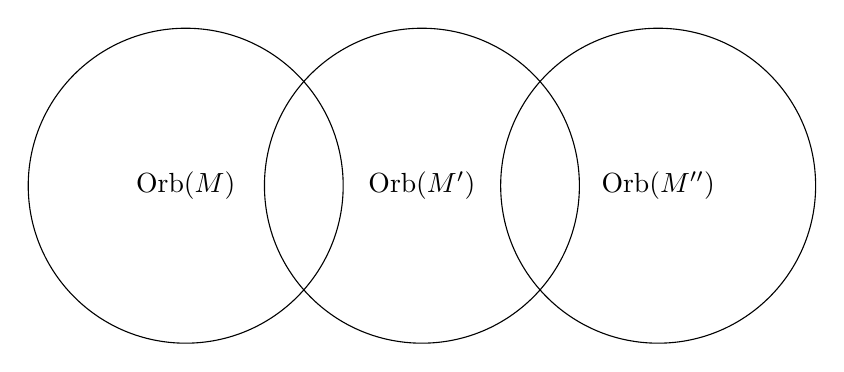
\begin{tikzpicture}[baseline=-0.25cm]
\draw (-3,0) circle (2) (-3,0)  node [text=black] {$\textnormal{Orb}(M)$};
\draw (0,0) circle (2) (0,0)  node [text=black] {$\textnormal{Orb}(M')$};
\draw (3,0) circle (2) (3,0) node [text=black] {$\textnormal{Orb}(M'')$};
\end{tikzpicture}.
\end{center}
\noindent\\ This picture becomes much more insightful in light of \hyperref[ActionPreorder]{Lemma \ref*{ActionPreorder}} and \hyperref[Transitive2]{Proposition \ref*{Transitive2}}.\\

%\noindent\textcolor{red}{Transitivity seems to be a stronger condition than being indecomposable. Note that being indecomposable means that, given any object $M \in \obset(\mathcal{M})$, we can

% In order to show that indecomposable implies transitive, we would need to be able to show that the orbit $\textnormal{Orb}(M)$ of each object $M \in \obset(\mathcal{M})$ cannot overlap with $\textnormal{Orb}(M')$ of any $M' \in \obset(\mathcal{M})\setminus\obset(\textnormal{Orb}(M))$, except at zero; that is, orbits are either disjoint or they coincide. Then we can use contradiction.}\\

\noindent\begin{definition}\textnormal{($\mathscr{C}$-Stable Ideal).} Let $\textnormal{M}$ be a birepresentation of $\mathscr{C}$. A %{\em left} (respectively {\em right}, {\em two-sided})
{\em $\mathscr{C}$-stable ideal} $\textnormal{I}$ of $\textnormal{M}$ is a collection $\textnormal{I} \coloneqq \{\textnormal{I}(\textobj{i}) : \textobj{i} \in \obset(\mathscr{C})\}$, where each $\textnormal{I}(\textobj{i})$ is a %left (respectively right, two-sided)
two-sided ideal of $\textnormal{M}(\textobj{i})$ such that $[\textnormal{M}(F)](\textnormal{I}(\textobj{i}))$ is a subclass of $\textnormal{I}(\textobj{j})$ for all $1$-morphisms $F \in \morset_\mathscr{C}^1(\textobj{i}, \textobj{j})$. %, for any morphism $\eta \in \textnormal{I}(\textobj{i})$ and any $1$-morphism $F \in \morset_\mathscr{C}^1(\textobj{i}, \textobj{j})$, we have that $[\textnormal{M}(F)](\eta) \in \textnormal{I}(\textobj{j})$.
%We say that $\textnormal{I}$ is {\em trivial} if, for all $\textobj{i} \in \obset(\mathscr{C})$, we have that either $\textnormal{I}(\textobj{i}) = \{0\}$ or $\textnormal{I}(\textobj{i}) = \morset(\textnormal{M}(\textobj{i}))$.\\
A $\mathscr{C}$-stable subideal $\textnormal{I}$ of a $\mathscr{C}$-stable ideal $\textnormal{J}$ is a $\mathscr{C}$-stable ideal for which $\textnormal{I}(\textobj{i})$ is a subideal of $\textnormal{J}(\textobj{i})$ for all $\textobj{i} \in \obset(\mathscr{C})$. We say that $\textnormal{I}$ is {\em proper} if there exists some $\textobj{i} \in \obset(\mathscr{C})$ for which $\textnormal{I}(\textobj{i})$ is proper, and {\em maximal} if it is proper and not a $\mathscr{C}$-stable subideal of any other proper $\mathscr{C}$-stable ideal.\\
\end{definition}

\noindent\begin{definition}\textnormal{(Simple Birepresentation).} %A multifinitary birepresentation of a multifinitary bicategory $\mathscr{C}$ is said to be {\em simple} (or {\em simple transitive}) if all of its $\mathscr{C}$-stable ideals are trivial.\\
A multifinitary birepresentation of a multifinitary bicategory $\mathscr{C}$ is said to be {\em simple} if it admits no proper, non-zero $\mathscr{C}$-stable ideals.\\
\end{definition}

\noindent Similarly to before, we say that a $\mathcal{C}$-module category $\mathcal{M}$ is simple if its corresponding birepresentation is simple. In other words, given non-zero $f, g \in \morset(\mathcal{M})$, we can obtain $g$ by composing $f$ with other morphisms in $\mathcal{M}$ and acting via $\mathcal{C}$ (by taking the left monoidal product with identity morphisms).\\

\noindent In light of the module category picture, we see that the ``right'' way to think about transitivity and simplicity is to observe that transitivity is really just asking that your birepresentation is cyclically generated by its objects ($\textsf{add}(\{X \otimes M : X \in \obset(\mathcal{C})\}) = \obset(\mathcal{M})$ for all $X \in \obset(\mathcal{M})$), while simplicity is asking that it is cyclically generated by its morphisms ($\{g \otimes f : g \in \morset(\mathcal{C})\} = \morset(\mathcal{M})$ for all $f \in \morset(\mathcal{M})$)! This perspective, in addition to the following result, really elucidates our notion of simplicity for birepresentations.\newpage

%\noindent\textcolor{red}{Are there any well-known adjectives that transitive and simple are equivalent to? Is simple here the same as semisimple and indecomposable, the definition Pinhas uses? Probably not.}\\

\noindent\begin{proposition} Every simple birepresentation is transitive.\\
\end{proposition}

\noindent\begin{proof} %Let $\textnormal{M}$ be a simple birepresentation of a multifinitary bicategory $\mathscr{C}$ and take $X \in \obset(\textnormal{M}(\textobj{i}))$ non-zero. Certainly $\textnormal{G}_\textnormal{M}(\{X\})$ induces a $\mathscr{C}$-stable ideal of $\textnormal{M}$, so it must be trivial by simplicity. In other words, for all $\textobj{j} \in \obset(\mathscr{C})$, we know that $\mathscr{C}_\textobj{j}(\{X\})$ must either be the trivial category $\{0\}$ or equivalent to $\textnormal{M}(\textobj{j})$.
%\textcolor{red}{Why is this non-zero when $X$ is non-zero? Supposedly we need the proof for lemma 3 of https://www2.math.uu.se/~vomaz677/PREPRINTS/VANESSA/transit.pdf, but the relevance of this makes no sense to me.} This completes the proof.
Let $\textnormal{M}$ be a simple birepresentation of a multifinitary bicategory $\mathscr{C}$ and take $X \in \obset(\textnormal{M}(\textobj{i}))$ non-zero. Certainly $\textnormal{G}_\textnormal{M}(\{X\})$ is non-zero (as it contains $X$) and hence induces a non-proper $\mathscr{C}$-stable ideal of $\textnormal{M}$ by simplicity. Thus for each $\textobj{j} \in \obset(\mathscr{C})$, we know that $\morset(\mathscr{C}_\textobj{j}(\{X\}))$ cannot be proper and so $\mathscr{C}_\textobj{j}(\{X\})$ must be equivalent to $\textnormal{M}(\textobj{j})$. In other words, $\textnormal{M}$ is transitive. This completes the proof.
\end{proof}\\

\noindent It is not necessarily the case that transitive birepresentations are simple! Many of the Lusztig-Vogan module categories we will study are not simple, but they are all transitive. We do, however, have the following proposition. This result will end up being important in formulating the categorical version of the Jordan--H\"{o}lder theorem.\\ %(see https://arxiv.org/abs/0808.0764)
%Recall from \hyperref[YonedaBirepresentation]{Example \ref*{YonedaBirepresentation}} the Yoneda $2$-representation for $\mathscr{C}$ the monoidal delooping of $\textsf{Vect}$. The action of $\textnormal{M}$ is given by the tensor product; that is, $[\textnormal{M}(V)](U) \coloneqq V \otimes U$. Thus $\mathbb{P}_\bullet$ is naturally transitive, as the additive subcategory of vector space $V \otimes U$, for any non-zero vector spaces $V$ and $U$, is simply $\textsf{Vect}$. However, it is certainly not simple! To see why, suppose we let $A$ be any non-invertible two-dimensional matrix, and $\mathcal{I}(\mathbbm{k}^2, \mathbbm{k}^2)$ the algebra ideal generated by $A$. It's easy to see that this generates a proper, non-zero $\mathscr{C}$-stable ideal. \textcolor{red}{Pretty sure this is correct but it feels too easy, double check it!}\\

%\noindent\begin{proposition} A module category corresponds to a simple birepresentation if and only if \textcolor{red}{...}.\\
%\end{proposition}

%\noindent\begin{proof}
%\end{proof}\\

%\noindent Let $\mathscr{C}$ be a multifinitary bicategory and denote by $\mathcal{S}(\mathscr{C})$ the multisemigroup of isomorphism classes of $1$-morphisms in $\mathscr{C}$, as per \cite[section 3.3]{MM14}. We define on $\mathcal{S}(\mathscr{C})$ a left preorder $\geq_L$ by saying, for two $1$-morphisms $F, G \in \morset^1(\mathscr{C})$, that $F \geq_L G$ if and only if there is a $1$-morphism $H \in \morset^1(\mathscr{C})$ for which $F$ is isomorphic to a direct summand of $H \circ G$. We define an equivalence relation $\sim$ given by $F \sim G$ if and only if $F \geq_L G$ and $G \geq_L F$, and call equivalence classes under this relation {\em left cells}.\\

%\noindent Given some left cell $\mathcal{L}$ in $\mathscr{C}$, let $\textobj{i} \in \obset(\mathscr{C})$ be the object that is the domain for every $1$-morphism in $\mathcal{L}$. Moreover, for $\textobj{j} \in \obset(\mathscr{C})$, let $\textnormal{N}(\textobj{j})$ denote the additive closure in $\mathbb{P}_\textobj{i}(\textobj{j})$ of all $1$-morphisms $F \in \mathscr{C}(\textobj{i}, \textobj{j})$ for which $F \geq_L \mathcal{L}$. This induces a finitary sub-birepresentation of $\mathbb{P}_\textobj{i}$ given by $\textnormal{N} : \textobj{j} \mapsto \textnormal{N}(\textobj{j})$.\\

%%%%%%%%%%%%%%%%%%%%%%%%%%%%%%%%%%%%%%%%%%%%%%%%%%
%%%%%%%%%%%%%%%%%%%%%%%%%%%%%%%%%%%%%%%%%%%%%%%%%%

%\noindent\begin{remark}\label{MatrixCalculus} Let $\mathcal{C}$ be an additive category. Then by \cite[\S VIII.2]{Mac13}, its morphisms form a matrix calculus; that is, for any $f \in \morset_\mathcal{C}(X, Y)$ with $X \cong \bigoplus_{i=1}^m{X_i}$ and $Y \cong \bigoplus_{j=1}^n{Y_j}$, we have that
%\begin{align*}
%\begin{split}
%f = \sum_{j=1}^n{\sum_{i=1}^m{(\iota_{Y_j} \circ f_{i,j} \circ \pi_{X_i})}}
%\end{split}
%\end{align*}
%\noindent for $f_{i,j} \coloneqq \pi_{Y_j} \circ f \circ \iota_{X_i}$, where $\pi_{X_i} : X \to X_i$ and $\pi_{Y_j} : Y \to Y_j$ are epimorphisms while $\iota_{X_i} : X_i \to X$ and\linebreak $\iota_{Y_j} : Y_j \to Y$ are monomorphisms for all $i \in \{1, \dots, m\}$ and $j \in \{1, \dots, n\}$.\\
%\end{remark}

%%%%%%%%%%%%%%%%%%%%%%%%%%%%%%%%%%%%%%%%%%%%%%%%%%
%%%%%%%%%%%%%%%%%%%%%%%%%%%%%%%%%%%%%%%%%%%%%%%%%%

%\noindent\begin{proposition} There is a unique maximal $\mathscr{C}$-stable ideal $\textnormal{I}$ in $\textnormal{N}$. Moreover, no $\textnormal{N}(\textobj{i})$ contains the identity morphism $\textnormal{id}_F$ for any $F \in \mathcal{L}$.\\
%\end{proposition}

\noindent\begin{proposition}\label{UniqueMaximalIdeal} Let $\textnormal{M}$ be a transitive birepresentation of a multifinitary bicategory $\mathscr{C}$. Then $\textnormal{M}$ admits a unique maximal $\mathscr{C}$-stable ideal $\textnormal{I}$, and moreover each $\textnormal{I}(\textobj{i})$ contains no identity morphisms apart from the one corresponding to the zero object.\\
\end{proposition}

\noindent\begin{proof} Let $\textnormal{I}$ be the sum (as vector spaces) of all $\mathscr{C}$-stable ideals of $\textnormal{M}$ that do not contain $\textnormal{id}_X$ for any non-zero $X \in \obset(\textnormal{M}(\textobj{i}))$ and any $\textobj{i} \in \obset(\mathscr{C})$. This is certainly itself a $\mathscr{C}$-stable ideal by construction. Moreover, because $U, V \subseteq U + V$ for vector spaces $U, V$, it follows that a sum of ideals is itself an ideal containing each ideal being summed, whence $\textnormal{I}$ is maximal with respect to $\mathscr{C}$-stable ideals not containing identity morphisms. To see that it is genuinely maximal, suppose $\textnormal{J}$ is a $\mathscr{C}$-stable ideal containing $\textnormal{I}$. %We first note that by \hyperref[MatrixCalculus]{Remark \ref*{MatrixCalculus}}, each $\textnormal{J}(\textobj{i})$ will be uniquely determined by its morphisms between indecomposable objects, so we may restrict our focus to such morphisms.
Because $\textnormal{I}$ is maximal with respect to $\mathscr{C}$-stable ideals not containing identity morphisms, $\textnormal{J}$ must contain at least one identity morphism, say $\textnormal{id}_X$ for some non-zero $X \in \obset(\textnormal{M}(\textobj{i}))$. Given any non-zero $Y \in \obset(\textnormal{M}(\textobj{j}))$, the transitivity of $\textnormal{M}$ tells us that $Y$ is either isomorphic to a direct summand of $[\textnormal{M}(F)](X)$, for some $F \in \morset_\mathcal{C}^1(\textobj{i}, \textobj{j})$, or isomorphic to a direct sum $[\textnormal{M}(F_1)](X) \oplus \cdots \oplus [\textnormal{M}(F_n)](X)$, for some $F_1, \dots, F_n \in \morset_\mathcal{C}^1(\textobj{i}, \textobj{j})$. We claim that $\textnormal{id}_Y$ must lie in $\textnormal{J}(\textobj{j})$ in both cases.\\[-1.5\baselineskip]
\begin{center}
\rule{0.5\linewidth}{1pt}
\end{center}
\noindent\\[-\baselineskip]
\noindent Let $F \in \morset_\mathcal{C}^1(\textobj{i}, \textobj{j})$ with $[\textnormal{M}(F)](X) = X_1 \oplus \cdots \oplus X_n$ and suppose that $\varphi : Y \to X_k$ is an isomorphism for some $1 \leq k \leq n$. Then $[\textnormal{M}(F)](\textnormal{id}_X) = \textnormal{id}_{X_1 \oplus \cdots \oplus X_n} \in \textnormal{J}(\textobj{j})$ by $\mathscr{C}$-stability. But by pre-composing with $\iota_{X_k} \circ \varphi^{-1} : Y \to X_k \to X_1 \oplus \cdots \oplus X_n$ and post-composing with $\varphi \circ \pi_{X_k} : X_1 \oplus \cdots \oplus X_n \to X_k \to Y$, we obtain that $\textnormal{id}_Y = (\varphi \circ \pi_{X_k}) \circ \textnormal{id}_{X_1 \oplus \cdots \oplus X_n} \circ (\iota_{X_k} \circ \varphi^{-1}) \in \textnormal{J}(\textobj{j})$.\\[-1.5\baselineskip]
\begin{center}
\rule{0.5\linewidth}{1pt}
\end{center}
\noindent\\[-\baselineskip]
\noindent Suppose now that $\varphi : Y \to X_1 \oplus \cdots \oplus X_n$ is an isomorphism, where for each  $1 \leq k \leq n$ we have $X_k = [\textnormal{M}(F_k)](X)$ for some $F_k \in \morset_\mathcal{C}^1(\textobj{i}, \textobj{j})$. As before, $[\textnormal{M}(F_k)](\textnormal{id}_X) = \textnormal{id}_{X_k} \in \textnormal{J}(\textobj{j})$ for all $1 \leq k \leq n$ by $\mathscr{C}$-stability. Moreover, because $\textnormal{J}(\textobj{j})$ is an ideal, $\iota_{X_k} \circ \textnormal{id}_{X_k} \circ \pi_{X_k} = \iota_{X_k} \circ \pi_{X_k} \in \textnormal{J}(\textobj{j})$ for all $1 \leq k \leq n$. Thus by the definition of an additive category, $\textnormal{id}_{X_1 \oplus \cdots \oplus X_n} = \iota_{X_1} \circ \pi_{X_1} + \cdots + \iota_{X_n} \circ \pi_{X_n} \in \textnormal{J}(\textobj{j})$, whence it follows that $\textnormal{id}_Y = \varphi^{-1} \circ \textnormal{id}_{X_1 \oplus \cdots \oplus X_n} \circ \varphi \in \textnormal{J}(\textobj{j})$.\\[-1.5\baselineskip]
\begin{center}
\rule{0.5\linewidth}{1pt}
\end{center}
\noindent\\[-\baselineskip]
\noindent We have thus shown that $\textnormal{J}$ must contain {\em all} identity morphisms and therefore cannot be proper, meaning that $\textnormal{I}$ must in fact be maximal as claimed. The uniqueness of $\textnormal{I}$ follows by construction. This completes the proof.
%We claim that this $\mathscr{C}$-stable ideal is not only maximal, but the unique maximal ideal not containing non-zero identity morphisms. First, by \hyperref[MatrixCalculus]{Remark \ref*{MatrixCalculus}}, each $\textnormal{I}(\textobj{i})$ will be uniquely determined by its morphisms between indecomposable objects. Suppose therefore that we have some indecomposable $X \in \obset(\textnormal{M}(\textobj{i}))$; naturally, the corresponding unital algebra $\textnormal{End}_{\textnormal{M}(\textobj{i})}(X)$ of endomorphisms of $X$ is local by \hyperref[KrullSchmidt]{Theorem \ref*{KrullSchmidt}}. In other words, it admits a unique maximal ideal $J(X)$, known as the Jacobson radical. This ideal consists of all non-invertible elements of $\textnormal{End}_{\textnormal{M}(\textobj{i})}(X)$, and hence is the largest ideal that does not contain $\textnormal{id}_X$. But now we know that if we have any subideals of $J(X)$, then they are all subideals of their sum, which remains a subideal of $J(X)$; in other words, by extending this logic to every indecomposable object, we see that $\textnormal{I}$ is certainly maximal and does not contain any identity morphisms. That $\textnormal{I}$ is the unique $\mathscr{C}$-stable ideal with these properties follows directly from the uniqueness of each $J(X)$. This completes the proof.
\end{proof}\newpage

\noindent\begin{definition}\!\textnormal{(Quotient Category).}\label{QuotientCategory } Let $\mathcal{C}$ be a $\mathbbm{k}$-linear category admitting a two-sided ideal $\mathcal{I}$. We define the {\em quotient category} $\mathcal{C}/\mathcal{I}$ to be the subcategory whose classes of morphisms are given by $\mathcal{C}/\mathcal{I}(X, Y) \coloneqq \mathcal{C}(X, Y)/\mathcal{I}(X, Y)$, for all $X, Y \in \obset(\mathcal{C})$, and whose objects are those objects $X \in \obset(\mathcal{C})$ for which $\textnormal{id}_X \in \mathcal{C}/\mathcal{I}(X, X)$ (that is, for which $\mathcal{C}/\mathcal{I}(X, X) \neq \varnothing$).\\
\end{definition}

\noindent\begin{propositiondefinition}\!\textnormal{(Simple Quotient).}\label{SimpleQuotient} \!A transitive birepresentation $\textnormal{M}$ of a %\linebreak
multifinitary bicategory $\mathscr{C}$ is simple if and only if the unique maximal $\mathscr{C}$-stable ideal $\textnormal{I}$ from \hyperref[UniqueMaximalIdeal]{Proposition \ref*{UniqueMaximalIdeal}} is the zero ideal. The simple sub-birepresentation $\underline{\textnormal{M}}$ of $\textnormal{M}$ that sends each object $\textobj{i} \in \obset(\mathscr{C})$ to the quotient subcategory $\textnormal{M}(\textobj{i})/\textnormal{I}(\textobj{i})$ is known as the {\em simple quotient} of $\textnormal{M}$.\\
\end{propositiondefinition}

\noindent\begin{proof} Naturally if $\textnormal{I}$ -- the sum of all $\mathscr{C}$-stable ideals without non-zero identity morphisms -- is the zero ideal, then $\textnormal{M}$ must contain no proper, non-zero $\mathscr{C}$-stable ideals. Conversely, if $\textnormal{M}$ is simple, then because $\textnormal{I}$ is the sum of proper $\mathscr{C}$-stable ideals, they must all be zero. Finally, because $\textnormal{I}$ is maximal, every morphism $f \in \morset(\textnormal{M}(\textobj{i})/\textnormal{I}(\textobj{i}))$ must generate either $\{0\}$ or $\textnormal{M}(\textobj{i})/\textnormal{I}(\textobj{i})$ under multiplication by $\mathscr{C}$, whence it follows that $\underline{\textnormal{M}}$ is simple. This completes the proof.
\end{proof}\\

\noindent Let $\textnormal{M}$ be a multifinitary birepresentation of $\mathscr{C}$. We denote by $\textnormal{Ind}(\textnormal{M})$ the set of isomorphism classes of indecomposable objects in every $\textnormal{M}(\textobj{i})$, for $\textobj{i} \in \obset(\mathscr{C})$; that is,
\begin{align*}
\begin{split}
\textnormal{Ind}(\textnormal{M}) = \bigsqcup_{\textobj{i} \in \obset(\mathscr{C})} \{[X] \in \textnormal{M}(\textobj{i}) : \textnormal{$X$ is indecomposable}\}.
\end{split}
\end{align*}
\noindent Note that $\textnormal{Ind}(\textnormal{M})$ is clearly finite, as $\mathscr{C}$ has finitely many objects and each category $\textnormal{M}(\textobj{i}) \in \obset(\mathfrak{A}_\mathbbm{k}^f)$ has finitely many isomorphism classes of indecomposable objects.\\

\noindent For $X, Y \in \textnormal{Ind}(\textnormal{M})$, where for instance $X \in \textnormal{M}(\textobj{i}_X)$ and $Y \in \textnormal{M}(\textobj{i}_Y)$, we write $X \geq Y$ if there exists a $1$-morphism $F \in \morset_\mathscr{C}^1(\textobj{i}_X, \textobj{i}_Y)$ such that $X$ is isomorphic to a direct summand of $[\textnormal{M}(F)](Y)$.\\

\noindent\begin{lemma}\label{ActionPreorder} Let $\textnormal{M}$ be a multifinitary birepresentation. The binary relation $\geq$ defined above defines a preorder on $\textnormal{Ind}(\textnormal{M})$ known as the {\em action preorder}.\\
\end{lemma}

\noindent\begin{proof} Clearly $\geq$ is reflexive, as we can just take $F \coloneqq \textnormal{id}_\textobj{i}$. Moreover, suppose that $X$ is isomorphic to a direct summand of $[\textnormal{M}(F)](Y)$ and $Y$ is isomorphic to a direct summand of $[\textnormal{M}(G)](Z)$; that is,
\begin{align*}
\begin{split}
[\textnormal{M}(F)](Y) &\cong X \oplus X_1 \oplus X_2 \oplus \cdots,\\
[\textnormal{M}(G)](Z) &\cong Y \oplus Y_1 \oplus Y_2 \oplus \cdots.
\end{split}
\end{align*}
\noindent In order to show transitivity, we would like to show that $X$ is isomorphic to a direct summand of $[\textnormal{M}(FG)](Z)$. Well, because the morphisms of $\mathfrak{A}_\mathbbm{k}^f$ are additive, we simply observe that
\begin{align*}
\begin{split}
[\textnormal{M}(FG)](Z) &\cong [\textnormal{M}(F)](Y) \oplus [\textnormal{M}(F)](Y_1) \oplus [M(F)](Y_2) \oplus \cdots\\
&\cong X \oplus X_1 \oplus X_2 \oplus \cdots \oplus [\textnormal{M}(F)](Y_1) \oplus [\textnormal{M}(F)](Y_2) \oplus \cdots.
\end{split}
\end{align*}
\noindent This completes the proof.
\end{proof}\\

\noindent Suppose we define an equivalence relation $\sim$ given by $X \sim Y$ if and only if $X \geq Y$ and $Y \geq X$. Obviously $\geq$ extends to a partial order on $\textnormal{Ind}(\textnormal{M})/\!\sim$. In particular, we have the following result.\newpage

\noindent\begin{proposition}\label{Transitive2} Let $\textnormal{M}$ be a multifinitary birepresentation. Then $\textnormal{M}$ is transitive if and only if\linebreak $\textnormal{Ind}(\textnormal{M})/\!\sim$ has only one element.\\
\end{proposition}

\noindent\begin{proof} Suppose $\textnormal{Ind}(\textnormal{M})/\!\sim$ is a singleton and take any $X \in \obset(\textnormal{M}(\textobj{i}))$ non-zero as a representative. Then for any indecomposable $Y \in \obset(\textnormal{M}(\textobj{j}))$, there exists some $F \in \morset_\mathscr{C}^1(\textobj{i}, \textobj{j})$ for which $Y$ is isomorphic to a direct summand of $[M(F)](X)$, since $Y \geq X$. In other words, the additive subcategory $\mathscr{C}_\textobj{j}(\{X\})$ is equivalent to $\textnormal{M}(\textobj{j})$, as by definition it is closed under direct summands. Thus $\textnormal{M}$ is transitive.\\[-1.5\baselineskip]
\begin{center}
\rule{0.5\linewidth}{1pt}
\end{center}
\noindent\\[-\baselineskip]
\noindent Conversely, suppose $\textnormal{M}$ is transitive, and consider any pair of indecomposables $X \in \obset(\textnormal{M}(\textobj{i}))$ and $Y \in \obset(\textnormal{M}(\textobj{j}))$. Because $\mathscr{C}_\textobj{j}(\{X\})$ is equivalent to $\textnormal{M}(\textobj{j})$, we know by the definition of $\mathscr{C}_\textobj{j}(\{X\})$ that $Y$ is isomorphic to a direct summand of $[M(F)](X)$ for some $F \in \morset_\mathscr{C}^1(\textobj{i}, \textobj{j})$; that is, $Y \geq X$. The same argument applied to $\mathscr{C}_\textobj{i}(\{Y\})$ shows us that $X \geq Y$, whence $\textnormal{Ind}(\textnormal{M})/\!\sim$ has only one element. This completes the proof.
\end{proof}\\

\noindent\begin{definition}\textnormal{(Directed Order Ideal).} A {\em directed order coideal} of a partially ordered set $(P, \geq)$ is a non-empty subset $I$ such that
\begin{enumerate}[label=$\bullet$, leftmargin=4\parindent]
\item for all $x \in I$ and $y \in P$, $y \geq x$ implies that $y \in I$ (upper set);
\item for all $x, y \in I$, there is some $z \in I$ such that $x \geq z$ and $y \geq z$ (downward directed set).\\
\end{enumerate}
%\noindent A {\em coideal} of a partially ordered set $(P, \leq)$ is a subset that is an upper set and a downward directed set.\\
\end{definition}

\noindent\begin{remark} This definition is slightly unusual. It is more typical to talk of {\em directed order ideals} of partially ordered sets $(P, \leq)$, which are non-empty subsets that are lower sets and upward directed sets. We have chosen to use coideals rather than ideals due to how we have defined our partial order; the standard notion of a directed order ideal goes ``downwards'', while we want to go ``upwards''. To more explicitly illustrate why we have made this choice, suppose we have some $\mathcal{C}$-module category of $R$-modules with indecomposables $R, X \in \obset(\mathcal{C})$. Naturally we would expect $X \geq R$, and indeed with our setup this will be true, as we can always consider the functor $\textnormal{M}(X) = X \otimes_R -$.\\
%The reasoning behind this somewhat quirky setup will hopefully become clear once we look at some explicit examples of Jordan--H\"{o}lder filtrations.\\
%In the literature, this partial order is often written as $X \geq Y$ if there exists a $1$-morphism $F \in \morset_\mathscr{C}^1(\textobj{i}_Y, \textobj{i}_X)$ such that $X$ is isomorphic to a direct summand of $[\textnormal{M}(F)](Y)$; that is, the inequality symbol is the other way around. As a result, they consider {\em coideals} (non-empty subsets that are upper sets and downward directed sets) rather than ideals in what follows. This is because we want to go ``downwards'', in the sense that we collect all direct summands. \textcolor{red}{Why do they define the order ``backwards''? Is there some (cell?) interpretation for which that is more natural?}\\
\end{remark}

%\noindent\textcolor{red}{For what follows, we will be considering coideals rather than ideals; the reason is because we want to ``go upwards'' with respect to our equivalence relation. That is, if we have (the isomorphism class of) an indecomposable object $X$, we also want to have every object that, roughly speaking, is isomorphic to a direct summand of $X$ (perhaps after $X$ is acted on by $\mathscr{C}$). This ensures that we are closed under taking direct summands, even after an action by $\mathscr{C}$.}\newpage

\noindent Let $\textnormal{M}$ be a multifinitary birepresentation of $\mathscr{C}$ and $Q$ a directed order coideal of $\textnormal{Ind}(\textnormal{M})/\!\sim$. For $\textobj{i} \in \obset(\mathscr{C})$, define $\textnormal{M}_Q(\textobj{i})$ to be the additive subcategory of $\textnormal{M}(\textobj{i})$ generated by the indecomposable objects $X \in \obset(\textnormal{M}(\textobj{i}))$ whose equivalence class lies in $Q$. Then $\textnormal{M}_Q : \textobj{i} \mapsto \textnormal{M}_Q(\textobj{i})$ induces a multifinitary sub-birepresentation of $\textnormal{M}$, known as the sub-birepresentation of $\textnormal{M}$ associated to $Q$.\\

\noindent Let $Q \subset R$ be a pair of directed order coideals in $\textnormal{Ind}(\textnormal{M})/\!\sim$ and let $\textnormal{I}_Q(\textobj{i})$ denote the ideal in $\textnormal{M}_R(\textobj{i})$ generated by the identity morphisms in $\textnormal{M}_Q(\textobj{i})$, for $\textobj{i} \in \obset(\mathscr{C})$. This collection of ideals is $\mathscr{C}$-stable, whence the multifinitary birepresentation $\textnormal{M}_R$ induces a multifinitary birepresentation $\textnormal{M}_{R/Q} : \textobj{i} \mapsto \textnormal{M}_R(\textobj{i})/\textnormal{I}_Q(\textobj{i})$. This is known as the quotient of $\textnormal{M}$ associated to $Q \subset R$. Note that if $\abs{R \setminus Q} = 1$, then $\abs{\textnormal{Ind}(\textnormal{M}_{R/Q})/\!\sim} = 1$, so $\textnormal{M}_{R/Q}$ will be transitive by \hyperref[Transitive2]{Proposition \ref*{Transitive2}}.\\

\noindent Choose $r \in \textnormal{Ind}(\textnormal{M})/\!\sim$ and let $X_r$ be the maximal directed order coideal in $\textnormal{Ind}(\textnormal{M})/\!\sim$ that does not contain $r$. In other words, $(\textnormal{Ind}(\textnormal{M})/\!\sim)\setminus X_r$ -- the complement of $X_r$ -- has maximal element $r$. %\textcolor{red}{Why do they also say $r$ is {\em minimal} in the complement of $X_r$ despite their order being backwards to mine?}
Thus we also obtain a directed order coideal $Y_r \coloneqq X_r \cup \{r\}$, as $r$ being maximal in the complement means $Y_r$ will be an upper set, whence the associated quotient $\textnormal{M}_{Y_r/X_r}$ is transitive by \hyperref[Transitive2]{Proposition \ref*{Transitive2}}. We henceforth let $\underline{\textnormal{M}}_r$ denote the simple quotient $\underline{\textnormal{M}}_{Y_r/X_r}$.\newpage

%\noindent Before stating the main theorem of this section, we recall the classical Jordan-H\"{o}lder theorem for modules over rings. Let $M$ be an $R$-module admitting the two composition series
%\begin{align*}
%\begin{split}
%\{0\} = M_0 \subset M_1 \subset \cdots \subset M_n = M,%
%\end{split}
%\end{align*}
%%\noindent and
%\begin{align*}
%\begin{split}
%\{0\} = M_0' \subset M_1' \subset \cdots \subset M_m' = M,
%\end{split}
%\end{align*}
%\noindent where by {\em composition series} we mean that these are filtrations of submodules where the {\em composition factors} $L_i \coloneqq M_i/M_{i-1}$ and $L_i' \coloneqq M_j'/M_{j-1}'$ are simple for all $i \in \{1, \dots, n\}$ and $j \in \{1, \dots, m\}$. The {\em Jordan-H\"{o}lder theorem} tells us that the {\em composition lengths} are equal -- that is, $n = m$ -- and moreover that there exists a permutation $\sigma \in S_n$ such that $L_i \cong L_{\sigma(i)}'$ for all $i \in \{1, \dots, n\}$.\\

\noindent Consider a filtration of directed order coideals
\begin{align*}
\begin{split}
\varnothing = Q_0 \subset Q_1 \subset \cdots \subset Q_n = \textnormal{Ind}(\textnormal{M})/\!\sim
\end{split}
\end{align*}
\noindent such that $\abs{Q_i \setminus Q_{i-1}} = 1$ for all $i \in \{1, \dots, n\}$. We call this a {\em complete filtration}. As shown previously, from such a filtration we have a corresponding {\em weak Jordan-H\"{o}lder series}
\begin{align*}
\begin{split}
\{0\} = \textnormal{M}_{Q_0} \subset \textnormal{M}_{Q_1} \subset \cdots \subset \textnormal{M}_{Q_n} = \textnormal{M}
\end{split}
\end{align*}
\noindent consisting of sub-birepresentations whose {\em weak composition quotients} $\textnormal{L}_i \coloneqq \underline{\textnormal{M}}_{Q_i/Q_{i-1}}$ are simple birepresentations for all $i \in \{1, \dots, n\}$. With this, we have the following result.\\

\noindent\begin{theorem}\textnormal{(Weak Jordan--H\"{o}lder Theorem).} Let $\textnormal{M}$ be a multifinitary birepresentation of a\linebreak multifinitary bicategory $\mathscr{C}$ admitting the two complete filtrations
\begin{align*}
\begin{split}
\varnothing = Q_0 \subset Q_1 \subset \cdots \subset Q_n = \textnormal{Ind}(\textnormal{M})/\!\sim,%
\end{split}
\end{align*}
%\noindent and
\begin{align*}
\begin{split}
\varnothing = Q_0' \subset Q_1' \subset \cdots \subset Q_m' = \textnormal{Ind}(\textnormal{M})/\!\sim,
\end{split}
\end{align*}
\noindent with weak composition quotients $\{\textnormal{L}_i\}_{i=1}^n$ and $\{\textnormal{L}_j'\}_{j=1}^m$ respectively. Then $m = n$, and moreover there exists a permutation $\sigma \in S_n$ such that $\textnormal{L}_i$ and $\textnormal{L}_{\sigma(i)}$ are equivalent for all $i \in \{1, \dots, n\}$.\\
\end{theorem}

\noindent\begin{proof} We clearly have $m = n = \abs{\textnormal{Ind}(\textnormal{M})/\!\sim}$ by the definition of a complete filtration. Suppose now that $r \in \textnormal{Ind}(\textnormal{M})/\!\sim$; then there exist unique $i, j \in \{1, 2, \dots, n\}$ for which $Q_i\setminus Q_{i-1} = Q_j'\setminus Q_{j-1} = \{r\}$. If we can show that the birepresentations $\textnormal{L}_i$ and $\textnormal{L}_j'$ are both equivalent to $\underline{\textnormal{M}}_r$, then we are done. In particular, by symmetry it is enough to show that $\textnormal{L}_i$ is equivalent to $\underline{\textnormal{M}}_r$.\\[-1.5\baselineskip]
\begin{center}
\rule{0.5\linewidth}{1pt}
\end{center}
\noindent\\[-\baselineskip]
\noindent Let $\textnormal{I}_{X_r}$ be the $\mathscr{C}$-stable ideal in $\textnormal{M}_{Y_r}$ for which $\textnormal{M}_{Y_r/X_r} = \textnormal{M}_{Y_r}/\textnormal{I}_{X_r}$ and $\textnormal{I}_{Q_{i-1}}$ the $\mathscr{C}$-stable ideal in $\textnormal{M}_{Q_i}$ for which $\textnormal{M}_{Q_i/Q_{i-1}} = \textnormal{M}_{Q_i}/\textnormal{I}_{Q_{i-1}}$. Since $\{r\} = Q_i\setminus Q_{i-1}$, we know by construction that $Q_{i-1} \subseteq X_r$, as $X_r$ is by definition the maximal directed order coideal not containing $r$; similarly, $Q_i \subseteq Y_r$. This second inclusion induces a pseudonatural isomorphism from $\textnormal{M}_{Q_i}$ to $\textnormal{M}_{Y_r}$ (a collection of natural isomorphisms from functors between Hom-categories to functors between Hom-subcategories), whence the first inclusion induces a pseudonatural isomorphism $\sigma : \textnormal{M}_{Q_i} \Rightarrow \textnormal{M}_{Y_r/X_r}$ by taking the quotient. Now, $\textnormal{M}_{Q_i}/\textnormal{I}_{Q_{i-1}}$ contains only the objects generated by indecomposables in the equivalence class $r$. But for any such pair of indecomposable objects $X, Y \in \obset(\textnormal{M}(\textobj{j}))$ lying in the equivalence class $r$, we have that $\textnormal{I}_{X_r}(X, Y) \subseteq \textnormal{I}_{Q_{i-1}}(X, Y)$ by the aforementioned inequalities. Thus the pseudonatural isomorphism $\sigma$ factors through $\textnormal{M}_{Q_i/Q_{i-1}}$, in the sense that there exist pseudonatural transformations $\sigma_1 : \textnormal{M}_{Q_i} \Rightarrow \textnormal{M}_{Q_i/Q_{i-1}}$ and $\sigma_2 : \textnormal{M}_{Q_i/Q_{i-1}} \Rightarrow \textnormal{M}_{Y_r/X_r}$ such that $\sigma = \sigma_2 \circ \sigma_1$. In particular, this gives us a pseudonatural transformation $\sigma_2 : \textnormal{M}_{Q_i/Q_{i-1}} \Rightarrow \textnormal{M}_{Y_r/X_r}$ that is obviously surjective on morphisms by fullness; therefore, because $\textnormal{M}_{Q_i/Q_{i-1}}$ and $\textnormal{M}_{Y_r/X_r}$ are both transitive, taking their simple quotients via \hyperref[SimpleQuotient]{proposition \ref*{SimpleQuotient}} induces an equivalence between $\textnormal{L}_i$ and $\underline{\textnormal{M}}_r$ as desired, whence the result follows. This completes the proof.
\end{proof}\\

\noindent\textcolor{red}{This proof feels kind of handwavey, need to double-check it slowly. Also, in what sense is this weak Jordan-H\"{o}lder theorem ``weak''? The decategorifications of these simple quotients are ``transitive $\mathbb{N}$-modules'' and usually not simple. Should also do some examples here.}\\
\newpage

\ruledsection{Categories of Soergel Bimodules}{3}
\noindent\\ Throughout this chapter and the next, we will explore one of the main examples that has motivated the theory from the previous chapter: namely, categories of Soergel bimodules. The upshot is as follows. Given a Coxeter system $(W, S)$, we may define a corresponding Iwahori--Hecke algebra. These algebras appear all over mathematics, playing important roles in areas such as the representation theory of Lie groups and quantum groups, knot theory and statistical mechanics, among others. From this same Coxeter system, we may also construct a category of so-called Soergel bimodules, which is an algebraic categorification of the corresponding Iwahori--Hecke algebra. These categories were fundamental to the recent, purely algebraic proof of the {\em Kazhdan-Lusztig conjecture} (\cite[Conjecture 1.5]{KL79}) by Elias and Williamson (\cite{EW14}), and have since become an indispensable tool in Lie theory.\\
%First, however, we should provide some historical context. Our story starts in 1979, when Kazhdan and Lusztig introduced a family of polynomials arising from the Coxeter system corresponding to an Iwahori--Hecke algebra, now known as {\em Kazhdan--Lusztig polynomials}. They proposed that the algebraic characters of Verma modules -- certain representations of semisimple Lie algebras -- were related to the values of their associated Kazhdan--Lusztig polynomials at $1$ (\cite[Conjecture 1.5]{KL79}), hoping to address a\linebreak longstanding problem in representation theory. This conjecture came to be known as the\linebreak {\em Kazhdan--Lusztig conjecture}.\\

\noindent Before introducing categories of Soergel bimodules, we will briefly give definitions of Coxeter systems and Iwahori--Hecke algebras. We will not give much insight into these objects; for a more detailed survey, please see the wonderful book of Elias, Makisumi, Thiel and Williamson (\cite{EMTW20}).\\

\noindent\begin{definition}\textnormal{(Coxeter System).} Let $S$ be a finite set and $(m_{st})_{s,t \in S}$ a matrix satisfying
\begin{enumerate}[label=$\bullet$, leftmargin=4\parindent]
\item $m_{ss} = 1$, for each $s \in S$;
\item $m_{st} = m_{ts} \in \{2, 3, \dots\} \sqcup \{\infty\}$, for $s \neq t \in S$.
\end{enumerate}
%\begin{align*}
%\begin{split}
%m_{s,t} \in \begin{cases}\{1\},&s = t;\\\{2, 3, \dots\} \sqcup \{\infty\},&s \neq t.\end{cases}
%\end{split}
%\end{align*}
\noindent Consider now the subgroup $W$ of $F_S$, the free group over $S$, with presentation
\begin{align*}
\begin{split}
W &= \langle s \in S : \text{$(st)^{m_{st}} = 1$ for all $s, t \in S$ with $m_{st} < \infty$}\rangle.%\\
% &= \langle s \in S : \text{$s^2 = 1$, $(st)^{m_{st}} = (ts)^{m_{st}}$ for all $s, t \in S$ with $m_{st} < \infty$}\rangle.
\end{split}
\end{align*}
\noindent The pair $(W, S)$ is known as a {\em Coxeter system}, and any group $W$ admitting a Coxeter system is known as a {\em Coxeter group}.\\
\end{definition}

\noindent We call the generating set $S$ the set of {\em simple reflections} and $(m_{st})_{s,t \in S}$ a {\em Coxeter matrix}. Because $s^2 = 1$ for all $s \in S$, the relation $(st)^{m_{st}} = 1$ is equivalent to the braid relation $sts\cdots = tst\cdots$ for all $s, t \in S$ with $m_{st} < \infty$, where both sides are the product of $m_{st}$ simple reflections.\\

\noindent\begin{definition}\textnormal{(Expression).} Let $(W, S)$ be a Coxeter system with $w \in W$. An {\em expression for $w$ of length $k$} is any sequence $\underline{w} := (s_1, \dots, s_k)$, for some not necessarily unique choice of $s_1, \dots, s_k \in S$, such that $w = s_1 s_2 \cdots s_k$. The {\em length} of $w$, denoted $\ell(w)$, is the length of its shortest expression, and any expression for $w$ of length $\ell(w)$ is said to be {\em reduced}. Moreover, $\ell(w) = 0$ if and only if $w = 1$.\\
\end{definition}

\noindent\begin{theorem}\label{Matsumoto}\textnormal{(Matsumoto's Theorem).} For any two reduced expressions of an element of a Coxeter group, the first can always be transformed into the second by repeatedly applying the braid relation.\\
\end{theorem}

\noindent This result was first shown in \cite{Mat64}. A sketch is given in \cite[Theorem 2.20]{EMTW20}, and the full proof can be found in \cite[Theorem 1.2.2]{GP00}.\newpage

\noindent\begin{definition}\textnormal{(Iwahori--Hecke Algebra).} Let $(W, S)$ be a Coxeter system and $q$ a formal variable. The {\em (one-parameter) Iwahori--Hecke algebra} corresponding to $(W, S)$ is the unital, associative\linebreak $\mathbb{Z}[q, q^{-1}]$-algebra $\mathscr{H}(W, S)$ with generators $\{T_s : s \in S\}$ and relations
\begin{enumerate}[label=$\bullet$, leftmargin=4\parindent]
\item (braid relation) $T_sT_tT_s\cdots = T_tT_sT_t\cdots$ for all $s, t \in S$ with $m_{s,t} < \infty$, where both sides are the product of $m_{s,t}$ generators;
\item (quadratic relation) $(T_s - q^{-1})(T_s + q) = 0$, for all $s \in S$.\\
\end{enumerate}
\end{definition}

\noindent\begin{remark} If we identify our parameter $q$ with $1$, the Iwahori--Hecke algebra reduces to the group algebra $\mathbb{Z}W$. In other words, it is a deformation of the group algebra of its associated Coxeter group.\\
\end{remark}

\noindent\begin{remark} The one-parameter Iwahori--Hecke algebra is opposed to the more general\linebreak {\em multiparameter Iwahori--Hecke algebra}, where instead of taking $\mathscr{H}(W, S)$ to be over the ring of one-parameter Laurent polynomials $\mathbb{Z}[q, q^{-1}]$, we consider a {\em family} of units $\{q_s : s \in S\}$ and take $\mathscr{H}(W, S)$ to be over the ring $\mathbb{Z}[q_s^{\pm 1} : s \in S]$.\\
\end{remark}

\noindent Let $(W, S)$ be a Coxeter system, and take $(s_1, \dots, s_\ell)$ and $(t_1, \dots, t_\ell)$ to be two reduced expressions for $w \in W$. Then $T_{s_1}T_{s_2}\cdots T_{s_\ell} = T_{t_1}T_{t_2} \cdots T_{t_\ell} \eqqcolon T_w$ by \hyperref[Matsumoto]{Theorem \ref*{Matsumoto}} and the braid relation. In particular, by \cite[Theorem 3.5]{EMTW20}, the set $\{T_w : w \in W\}$ forms a $\mathbb{Z}[q, q^{-1}]$-basis for $\mathscr{H}(W, S)$ known as the {\em standard basis}. Another important basis is the Kazhdan--Lusztig basis.\\

\noindent\textcolor{red}{Kazhdan--Lusztig basis, change of basis from KL basis to standard basis is given by KL polynomials.}\\

\noindent\begin{definition}\textnormal{(Geometric Representation).} Let $(W, S)$ be a Coxeter system and $V$ the real vector space with basis $\{\alpha_s : s \in S\}$. Define a symmetric, bilinear form on $V$ by% = \textnormal{span}_\mathbb{R}(\{\alpha_s : s \in S\})$ by
\begin{align*}
\begin{split}
(\alpha_s, \alpha_t) = \begin{cases}-\cos\!\left(\frac{\pi}{m_{st}}\right)\!,&m_{s,t} \neq \infty;\\-1,&m_{s,t} = \infty.\end{cases}
\end{split}
\end{align*}
\noindent From this, we define an action of $s \in S$ on the basis elements $\alpha_t \in V$ by the linear automorphism
\begin{align*}
\begin{split}
s(\alpha_t) \coloneqq \alpha_t - 2(\alpha_s, \alpha_t)\alpha_s,
\end{split}
\end{align*}
\noindent which reflects $\alpha_t$ across $\alpha_s$. The {\em geometric representation} of $(W, S)$ is the representation induced by linearly extending this reflection action to an action of $W$ on all of $V$.\\
\end{definition}

\noindent\textcolor{red}{Try and explain the grading nonsense, then move on to Bott--Samelson bimodules and Soergel bimodules.}
\newpage

\noindent 

\newpage

\ruledsection{Lusztig--Vogan Module Categories}{4}
\noindent\\ This chapter will aim to summarize the recent work of Larson and Romanov in their Soergel bimodule approach for algebraically categorifying the trivial block of the Lusztig--Vogan module (\cite{LR22}), which provides interesting examples of module categories over the category of Soergel bimodules. In the most general setting, the construction of a Lusztig--Vogan module category takes as ingredients a connected, complex, reductive algebraic group $G$, a Borel subgroup $B$ of $G$, a holomorphic involution $\theta$ of $G$ and a finite-index subgroup $K$ of the fixed-point subgroup $G^\theta \coloneqq \{g \in G : \theta(g) = g\}$.\\

\noindent With the additional assumption that $K$ is the identity component of $G^\theta$ (see \cite{LR22} for details), we can proceed as follows. Let $P \coloneqq \textnormal{Sym}(\textnormal{span}_\mathbb{R}(X_*(T_K)))$ be the symmetric algebra on the $\mathbb{R}$-span of the cocharacter lattice of a maximal torus $T_K$ of $K$ contained in $B_K \coloneqq B \cap K$, graded such that $\textnormal{span}_\mathbb{R}(X_*(T_K))$ has degree $2$, and similarly let $R \coloneqq \textnormal{Sym}(\textnormal{span}_\mathbb{R}(X_*(T)))$ be the symmetric algebra on the $\mathbb{R}$-span of the cocharacter lattice of a maximal torus $T$ of $G$ contained in $B$, graded such that $\textnormal{span}_\mathbb{R}(X_*(T))$ has degree $2$. Denote by $W \coloneqq N_G(T)/T$ the Weyl group of $G$ corresponding to $T$, by $W^\theta$ the set of elements of $W$ fixed under the involution induced by $\theta$ and by $W_K \coloneqq N_K(T_K)/T_K$ the Weyl group of $K$ corresponding to $T_K$, where we write $P^{W_K} \coloneqq \{p \in P : wp = p\text{ for all }w \in W_K\}$. Note that $W_K \subseteq W^\theta \subseteq W$, and by choosing a set of simple roots in $W$ (using the positive roots corresponding to $B$) we obtain a Coxeter system $(W, S)$. Finally, let $\phi : R \to P$ be the algebra homomorphism extending the restriction map $X(T) \to X(T_K)$. For each $w \in W$, we define the {\em $w$-standard bimodule} $P_w$ to be the $(P_{W_K}, R)$-bimodule given by $P$ as a vector space with left action given by left multiplication and right action given by $s\cdot_w r \coloneqq s\phi(wr)$, for all $s \in P$ and $r \in R$. Define\\[-1.1\linespacing]
\begin{align*}
\begin{split}
\mathcal{N}_{LV}^0 \coloneqq \langle P_w \otimes_R X : w \in W^\theta, X \in \obset(\mathbb{S}\textcat{Bim}(W, S))\rangle_{\oplus,\ominus,(1)}
\end{split}
\end{align*}
\noindent to be the category of $(P^{W_K}, R)$-bimodules generated by standard bimodules under the right action of Soergel bimodules and closed under direct sums, direct summands and gradning shifts. By \cite[Theorem 1.3.1]{LR22}, this categorifies the trivial block of the associated module of Lusztig and Vogan.\\

\noindent To study this in full generality involves some deep results from Lie theory; thus for the time being we will restrict our attention to the case where the tori $T_K$ and $T$ are of equal rank (that is, where $T_K = T$ and hence $P = R$). In this situation the picture is much simpler. Let $(W, S)$ be a Coxeter system with finite index subgroup $W_K \subseteq W$. Given the collection $\{\alpha_s : s \in S\}$ of simple roots, we define a polynomial algebra $R \coloneqq \mathbb{R}[\alpha_1, \dots, \alpha_n]$, which we recall is isomorphic to the symmetric algebra of the vector space associated with the geometric representation of $(W, S)$. We therefore have an action of $W$ on $R$ induced by linearly extending the reflection action, given on generators $s \in W$ and simple roots $\alpha_t \in R$ by\\[-1.1\linespacing]
\begin{align*}
\begin{split}
s(\alpha_t) = \alpha_t + 2\cos\!\left(\frac{\pi}{m_{st}}\right)\!\alpha_s.
\end{split}
\end{align*}
\noindent\\[-0.6\linespacing] We define $R^{W_K}$ to be the polynomials in $R$ that are invariant under action by $W_K$. With this, given a generator $w$ representing a coset in $W/W_K$, we define the $w$-standard bimodule $R_w$ to be the $(R^{W_K}, R)$-bimdoule given by $R$ as a vector space with left action given by left multiplication and right action given by $s \cdot_w r \coloneqq s \cdot w(r)$, for all $s \in R_w$ and $r \in R$. Thus, just as before, the corresponding algebraic Lusztig--Vogan module category is
\begin{align*}
\begin{split}
\mathcal{M}_{LV}^0 = \langle R_w \otimes_R X : [w] \in W/W_K, X \in \obset(\mathbb{S}\textcat{Bim}(W, S))\rangle_{\oplus,\ominus,(1)}.
\end{split}
\end{align*}
\newpage

\noindent\begin{remark}\label{CartanInvolution} Suppose $G$ is a connected, complex, reductive algebraic group and let $\sigma : G \to G$ be an antiholomorphic involution of $G$. Then $G^\sigma$, the fixed-point subgroup of $\sigma$, has the structure of a real Lie group whose complexification is $G$. Moreover, $\sigma'$ is $G$-conjugate to $\sigma$ (that is, there exists some $h \in G$ for which $\sigma' = \textnormal{int}_h\circ\sigma\circ\textnormal{int}_h^{-1}$, where $\textnormal{int}_h : g \mapsto hgh^{-1}$ is known as the {\em inner automorphism associated to $h$}) if and only if $G^{\sigma'}$ and $G^\sigma$ are isomorphic as real Lie groups. We will call such an isomorphism class a {\em real form} of $G$. Now, a classical result of Cartan tells us the following. First, a connected, complex algebraic group is reductive if and only if it is the complexification of a unique connected, compact, real Lie group (\cite[p.\ 34]{Kam11}); thus there is, up to $G$-conjugation, only one antiholomorphic involution $\sigma_c$ whose fixed-point subgroup is compact. This is known as the {\em compact form} of $G$. Second, let $\Theta$ be any $G$-conjugacy class of holomorphic involutions of $G$. Then there exists some holomorphic involution $\theta \in \Theta$ that commutes with $\sigma_c$, and furthermore each $G$-conjugacy class of antiholomorphic involutions of $G$ contains $\sigma = \theta \circ \sigma_c$ for some unique choice of initial $\Theta$ (\cite{Ada14}). Putting everything together, we have bijections
\begin{align*}
\begin{split}
\{\text{real forms of $G$}\}\ \longleftrightarrow\ \left\{\begin{matrix}\text{antiholomorphic}\\\text{involutions of $G$}\end{matrix}\right\}\!\big/\!\!\sim\ \ \longleftrightarrow\ \left\{\begin{matrix}\text{holomorphic}\\\text{involutions of $G$}\end{matrix}\right\}\!\big/\!\!\sim,
\end{split}
\end{align*}
\noindent where the equivalence relations are given by conjugation by $G$. The holomorphic involution\linebreak corresponding to a real form is known as the {\em Cartan involution} of that real form. An immediate corollary is that a real form is compact if and only if its Cartan involution is the identity. For any real form, we also have a diamond
\begin{center}
\begin{tikzcd}
& G\arrow[dl, "\sigma"', no head]\arrow[dr, "\theta", no head] &\\
G_\mathbb{R} \coloneqq G^\sigma\arrow[dr, "\theta"', no head] && K \coloneqq G^\theta\arrow[dl, "\sigma", no head]\\
& K_\mathbb{R} \coloneqq G^{\sigma_c} &
\end{tikzcd}
\end{center}
\noindent where $G_\mathbb{R}$ is a real Lie group, $K$ is a complex Lie group and $K_\mathbb{R}$ is the maximal compact subgroup of $G_\mathbb{R}$. Note that $K$ is not in general compact, although it {\em will} be the complexification of $K_\mathbb{R}$.\\
\end{remark}




\noindent\begin{example} %Note that a complex algebraic group is reductive if and only if it is the\linebreak complexification of a unique connected, compact Lie group (\cite[p.\ 34]{Kam11}).
Let's work through an example with $G \coloneqq \textnormal{SL}(2, \mathbb{C})$. Recall that $G$ admits two real forms: a compact form $\textnormal{SU}(2)$ and a split form $\textnormal{SL}(2, \mathbb{R})$. The former is the fixed-point subgroup of the antiholomorphic involution $\sigma_c : g \mapsto ((\overline{g})^T)^{-1}$, while the latter is the fixed-point subgroup of the antiholomorphic involution $\sigma_s : g \mapsto \overline{g}$. By \hyperref[CartanInvolution]{Remark \ref*{CartanInvolution}}, the Cartan involution of $\textnormal{SU}(2)$ will be trivial; this is a bit boring, so let's look at $\textnormal{SL}(2, \mathbb{R})$ instead. It admits the Cartan involution $\theta' : g \mapsto (g^T)^{-1}$ with fixed-point subgroup
\begin{align*}
\begin{split}
G^{\theta'} = \textnormal{SO}(2, \mathbb{C}) \coloneqq \left\{\!\begin{pmatrix}\hphantom{-}a&b\\-b&a\end{pmatrix} : a, b \in \mathbb{C}, a^2 + b^2 = 1\right\}\!.
\end{split}
\end{align*}
\noindent Note that this is homeomorphic to $\mathbb{C}^\times \coloneqq \mathbb{C}\!\setminus\!\{0\}$ and is hence a maximal torus for $G$ as a complex algebraic group (that is, a subgroup that is maximal among subgroups homeomorphic to $(\mathbb{C}^\times)^{\oplus k}$), as there are no groups $H$ for which $G^{\theta'} \subset H \subset G$. In fact, it is the complexification of $\textnormal{SO}(2, \mathbb{R})$, the maximal torus of $\textnormal{SL}(2, \mathbb{R})$ as a real Lie group (that is, the subgroup that is maximal among subgroups homeomorphic to $(S^1)^{\oplus k}$). Since $G^{\theta'}$ is connected, the identity component is the entire group. However, $G^{\theta'}$ is awkward to work with; therefore, instead of using $G^{\theta'}$, consider the following.\newpage

\noindent Suppose we conjugate $\theta'$ by the inner automorphism associated to the matrix
\begin{align*}
\begin{split}
h \coloneqq \frac{1}{\csqrt{2}}\begin{pmatrix}1&i\\i&1\end{pmatrix}\! \in \textnormal{SL}(2, \mathbb{C});
\end{split}
\end{align*}
\noindent that is, let $\theta \coloneqq \textnormal{int}_h\circ\theta'\circ\textnormal{int}_h^{-1}$. Realizing $\theta'$ as the inner automorphism of the matrix with $1$ and $-1$ on its off-diagonals, we have
\begin{align*}
\begin{split}
\theta\!\left(\!\begin{pmatrix}a&b\\c&d\end{pmatrix}\!\right)\! &\coloneqq \frac{1}{4}\begin{pmatrix}1&i\\i&1\end{pmatrix}\begin{pmatrix}\hphantom{-}0&1\\-1&0\end{pmatrix}\begin{pmatrix}\hphantom{-}1&-i\\-i&\hphantom{-}1\end{pmatrix}\begin{pmatrix}a&b\\c&d\end{pmatrix}\begin{pmatrix}1&i\\i&1\end{pmatrix}\begin{pmatrix}0&-1\\1&\hphantom{-}0\end{pmatrix}\begin{pmatrix}\hphantom{-}1&-i\\-i&\hphantom{-}1\end{pmatrix}\\
&\hphantom{\coloneqq}\nhphantom{=}= \begin{pmatrix}\hphantom{-}a&-b\\-c&\hphantom{-}d\end{pmatrix}\!.
\end{split}
\end{align*}
\noindent This holomorphic involution admits the fixed-point subgroup
\begin{align*}
\begin{split}
G^\theta = \left\{\!\begin{pmatrix}a&0\hphantom{{}^{-1}}\\0&a^{-1}\end{pmatrix} : a \in \mathbb{C}^\times\right\}\!,
\end{split}
\end{align*}
\noindent which is of course homeomorphic to $\mathbb{C}^\times$. Once again, since $G^\theta$ is connected, the identity component is just the entire group, and hence we will take $K \coloneqq G^\theta$. Once again, $G^\theta$ is a maximal torus, and is given by the intersection of the pair of opposite Borel groups
\begin{align*}
\begin{split}
B \coloneqq \left\{\!\begin{pmatrix}a&b\hphantom{{}^{-1}}\\0&a^{-1}\end{pmatrix} : a \in \mathbb{C}^\times, b \in \mathbb{C}\right\}\!\qquad\text{and}\qquad B' \coloneqq \left\{\!\begin{pmatrix}a&0\hphantom{{}^{-1}}\\b&a^{-1}\end{pmatrix} : a \in \mathbb{C}^\times, b \in \mathbb{C}\right\}\!.
\end{split}
\end{align*}
\noindent Therefore, let $T \coloneqq G^\theta$. The corresponding Weyl group is $W \coloneqq N_G(T)/T = S_2 = \{1, s\}$, since
\begin{align*}
\begin{split}
N_G(T) = \{g \in G : gtg^{-1} \in T, \textnormal{for all $t \in T$}\} = T \sqcup \left\{\!\begin{pmatrix}0&b\\-b^{-1}&0\end{pmatrix} : b \in \mathbb{C}^\times\!\right\}\!;
\end{split}
\end{align*}
\noindent similarly, $T_K \coloneqq T$ is obviously then a maximal torus in $K$, giving us $W_K \coloneqq N_K(T_K)/T_K = \{1\}$. The only choice of simple roots we can make is $S = \{s\}$, whence $R = \mathbb{R}[\alpha_{s}]$. The action of $W$ on $R$ is given by $1 : r \mapsto r$ and $s : r \mapsto -r$, for $r \in R$, giving us $R^{W_K} = R$ and an easy $(R^{W_K}, R)$-bimodule structure for $R$. This gives us a very explicit right module category $\mathcal{M}_{LV}^0$ over $\mathbb{S}\textcat{Bim}(W, S)$! A standard exercise we can now do is to compute the Jordan--H\"{o}lder filtrations of the corresponding birepresentation $\textnormal{M}$ that maps $\bullet$ to $\mathcal{M}_{LV}^0$ and $X \in \obset(\mathbb{S}\textcat{Bim}(W, S))$ to functors $- \otimes X$. \textcolor{red}{When $T = G^\theta$, don't we always have that $W^\theta = \{e\}$?}\\[-1.5\baselineskip]%; therefore it is easily seen to be multifinitary.\\[-1.5\baselineskip]
\begin{center}
\rule{0.5\linewidth}{1pt}
\end{center}
\noindent\\[-\baselineskip]
\noindent Recall that the indecomposable objects in $\mathbb{S}\textcat{Bim}(W, S)$ are given by Bott--Samelson bimodules of the form $B_w \coloneqq R \otimes_{R^w} R(1)$, for $w \in W$. Because module products distribute over direct sums, it follows that the indecomposables of $\mathcal{M}_{LV}^0$ are of the form $R_{w_1} \otimes_R B_{w_2}$, for $[w_1] \in W/W_K$ and $w_2 \in W$; that is, products of generators of $\mathcal{M}_{LV}^0$ with indecomposable Soergel bimodules. In our case with $\textnormal{SL}(2, \mathbb{C})$, we have four candidates, which are evaluated as follows:
\begin{alignat*}{2}
R_1 \otimes_R B_1 \cong (R\hphantom{{}_{s}} \otimes_R R) \otimes_R R(1) &\cong R,&\qquad R_1 \otimes_R B_{s} \cong (R\hphantom{{}_{s}} \otimes_R R) \otimes_{R^{s}} R(1) &\cong B_{s},\\
R_{s} \otimes_R B_1 \cong (R_{s} \otimes_R R) \otimes_R R(1) &\cong R_{s},&\qquad R_{s} \otimes_R B_{s} \cong (R_{s} \otimes_R R) \otimes_{R^{s}} R(1) &\cong B_{s},
\end{alignat*}
\noindent where we note that $R_1 \cong R \cong B_1$. Our three indecomposables are therefore $R$, $R_{s}$ and $B_{s}$. Of course, $B_{s} \geq R, R_{s}$, since $B_{s}$ is isomorphic to both $[\textnormal{M}(B_{s})](R) = R \otimes_R B_{s}$ and $[\textnormal{M}(B_{s})](R_{s}) = R_{s} \otimes_R B_{s}$; thus we obtain the two complete filtrations
\begin{align*}
\begin{split}
\{B_{s}\} \subset \{R_{s}, B_{s}\} \subset \{R, R_{s}, B_{s}\}\qquad\text{and}\qquad\{B_{s}\} \subset \{R, B_{s}\} \subset \{R, R_{s}, B_{s}\}.
\end{split}
\end{align*}
\newpage
\noindent It is immediately obvious that the corresponding weak composition quotients will be equivalent, so we will just compute them for the filtration given by $Q_1 \coloneqq \{B_{s}\}$, $Q_2 \coloneqq \{R_{s}, B_{s}\}$ and $Q_3 \coloneqq \{R, R_{s}, B_{s}\}$. Defining subcategories $\mathcal{M}_{Q_i} \coloneqq \langle q \otimes_R X : q \in Q_i, X \in \obset(\mathbb{S}\textcat{Bim}(W, S))\rangle_{\oplus,\ominus,(1)}$ and two-sided ideals $\mathcal{I}_{Q_i}$ of $\mathcal{M}_{LV}^0$, we are able to define the quotient subcategories
\begin{align*}
\begin{split}
\mathcal{M}_{Q_3/Q_2} \coloneqq \mathcal{M}_{Q_3}/\mathcal{I}_{Q_2} = \langle R\hphantom{{}_{s}} \otimes_R X : X \in \obset(\mathbb{S}\textcat{Bim}(W, S))\rangle_{\oplus,\ominus,(1)},\\
\mathcal{M}_{Q_2/Q_1} \coloneqq \mathcal{M}_{Q_2}/\mathcal{I}_{Q_1} = \langle R_{s} \otimes_R X : X \in \obset(\mathbb{S}\textcat{Bim}(W, S))\rangle_{\oplus,\ominus,(1)},\\
\mathcal{M}_{Q_1/Q_0} \coloneqq \mathcal{M}_{Q_1}/\mathcal{I}_{Q_0} = \langle B_{s} \otimes_R X : X \in \obset(\mathbb{S}\textcat{Bim}(W, S))\rangle_{\oplus,\ominus,(1)}.
\end{split}
\end{align*}
\noindent In order to compute the weak composition quotients, we must quotient our sub-birepresentations of the form $\textnormal{M}_{Q_i/Q_{i-1}} : \bullet \mapsto \mathcal{M}_{Q_i/Q_{i-1}}$ by the unique maximal $\mathbb{S}\textcat{Bim}(W, S)$-stable ideals given by \hyperref[UniqueMaximalIdeal]{Proposition \ref*{UniqueMaximalIdeal}}. \textcolor{red}{It would be nice to understand explicitly the weak composition quotients (i.e. what the maximal stable ideals look like as vector spaces, but this might be hard).}
\end{example}
%In other words, we can (and usually will) start with a Lie group $G_\mathbb{R}$. As a first example, let's start with $G_\mathbb{R} \coloneqq \textnormal{SL}(2, \mathbb{R})$, which admits the maximal compact subgroup $K_\mathbb{R} \coloneqq \textnormal{SO}(2)$ (this is also its maximal torus). The complexification of $G_\mathbb{R}$ is of course $G \coloneqq \textnormal{SL}(2, \mathbb{C})$, while the complexification of $K_\mathbb{R}$ is homeomorphic to the subgroup $K$ of diagonal matrices in $G$. A maximal torus $T$ for $G$ is the subgroup of diagonal matrices in $\textnormal{SU}(2)$, whence the Weyl group of $G$ is $W \coloneqq N_G(T)/T = \mathbb{Z}/2\mathbb{Z}$, as
%\begin{align*}
%\begin{split}
%N_G(T) = \{g \in G : gtg^{-1} \in T, \textnormal{for all $t \in T$}\} = T \sqcup \left\{\begin{pmatrix}0&1\\1&0\end{pmatrix}\right\}.
%\end{split}
%\end{align*}
%\noindent The Weyl group of $K$, meanwhile, is just the trivial group $W_K \coloneqq N_K(T_K)/T_K = \{0\}$.

%\noindent\begin{example} Note that a complex algebraic group is reductive if and only if it is the\linebreak complexification of a unique connected, compact Lie group (\cite[p.\ 34]{Kam11}). In other words, we can (and usually will) start with a Lie group $G_\mathbb{R}$. As a first example, let's start with $G_\mathbb{R} \coloneqq \textnormal{SL}(2, \mathbb{R})$, which admits the maximal compact subgroup $K_\mathbb{R} \coloneqq \textnormal{SO}(2)$ (this is also its maximal torus). The complexification of $G_\mathbb{R}$ is of course $G \coloneqq \textnormal{SL}(2, \mathbb{C})$, while the complexification of $K_\mathbb{R}$ is homeomorphic to the subgroup $K$ of diagonal matrices in $G$. A maximal torus $T$ for $G$ is the subgroup of diagonal matrices in $\textnormal{SU}(2)$, whence the Weyl group of $G$ is $W \coloneqq N_G(T)/T = \mathbb{Z}/2\mathbb{Z}$, as
%\begin{align*}
%\begin{split}
%N_G(T) = \{g \in G : gtg^{-1} \in T, \textnormal{for all $t \in T$}\} = T \sqcup \left\{\begin{pmatrix}0&1\\1&0\end{pmatrix}\right\}.
%\end{split}
%\end{align*}
%\noindent The Weyl group of $K$, meanwhile, is just the trivial group $W_K \coloneqq N_K(T_K)/T_K = \{0\}$.
%\end{example}
\newpage

\renewcommand\thesection{R}
\ruledsectionstar{References}{References}
\begingroup
\setlength{\emergencystretch}{.5em}
\printbibliography[heading=none]
\endgroup
\newpage

\vspace*{\fill}
\hfill Page intentionally left blank. \hfill
\vspace*{\fill}
\newpage

\phantomsection\addcontentsline{toc}{section}{Talks}
\noindent\\\textbf{Motivation}
\begin{enumerate}[label=$\bullet$, leftmargin=1\parindent]
\item What is finitary birepresentation theory? My take: a ``categorification'' of the representation theory of finite-dimensional algebras, arising from the study of knot invariants, tensor categories and operator algebras. In other words, Jones mathematics (lol).
\item Stealing some slogans from one of Dani's talks: representation theory is group theory in vector spaces, while birepresentation theory is group theory in linear categories.
\item Why is it important? Basically for (somehow) studying the fields I just mentioned. Hopefully by the end of this little series we can figure out the answer to this together.\\
\end{enumerate}

\noindent\textbf{Plan}
\begin{enumerate}[label=$\bullet$, leftmargin=1\parindent]
\item Today I'd like to introduce one of the main theorems of birepresentation theory: the ``weak Jordan- H\"{o}lder theorem''. This theorem is a nice (abstract) motivation for the classification of simple birepresentations.
\item In principle I'm not sure how helpful this talk will be. It will mostly be walking you through what I've been thinking about over the past couple of weeks. The main theorem is, I think, quite nice, but getting there will likely be dry. Next time I'd like to focus more on examples (especially Soergel bimodules and their classification) if I'm capable enough.
\item Addressing a question: why am I talking about birepresentations? The people were promised $2$-representations! In classifying $2$-representations of Soergel bimodules, it was quickly found that the language of $2$-representations was too restrictive. Later on in this series I will probably transition to $2$-representations, but at least in this talk I'd like to state things as generally as possible to avoid issues later on.
\item As a reminder to myself, I'd like to maintain a little definition bank so you guys can keep track of definitions.\\
\end{enumerate}

\noindent\textbf{Multifinitary Categories}
\begin{enumerate}[label=$\bullet$, leftmargin=1\parindent]
\item What are multifinitary $1$-categories? Add this to the definition bank.
\item In linear algebra, all idempotents split. Idempotent complete categories live somewhere between additive categories and Abelian categories. In particular, {\em all pseudo-Abelian categories are\linebreak idempotent complete!} These remarks are what ``unlocked'' idempotent completeness for me.
\item Examples of finitary categories (that I can't write down because I haven't prepared any concrete examples): (semi)groups and their representations, quantum groups and their categorifications, tensor categories, fusion categories, modular (tensor) categories, $2$-Kac-Moody categories, etc.
\item $\textsf{Vect}_\mathbbm{k}$ is a helpful example: $\begin{pmatrix}1&0\\0&0\end{pmatrix} = \begin{pmatrix}1\\0\end{pmatrix}\!\begin{pmatrix}1&0\end{pmatrix}$.
\item Maybe mention example 2.8? Mazorchuk and Miemietz would have you believe it's a useful example but man is it impenetrable.
\item Also, $\mathbb{S}\textsf{Bim}(W, S)$ lololol
\item Define the category of multifinitary categories.
\item Finitary bicategories. Add this to the definition bank. We can generate these from finitary monoidal categories: in particular, there is a bijection between monoidal categories and one-object bicategories, with delooping taking us upstairs and Hom-categories taking us downstairs. Mention strict case.
\end{enumerate}
\newpage

\noindent\textbf{Finitary Birepresentations}
\begin{enumerate}[label=$\bullet$, leftmargin=1\parindent]
\item What are finitary birepresentations? There is a bijection between module categories and\linebreak birepresentations of one-object bicategories. Example: Yoneda birepresentations.
\item Equivalence of birepresentations. I don't understand these very well yet.\\
\end{enumerate}

\noindent\textbf{Simple Birepresentations}
\begin{enumerate}[label=$\bullet$, leftmargin=1\parindent]
\item Walk through next block: essentially, I want to define what it means for a birepresentation to be transitive. If you're like me and you keep forgetting what this adjective means, an action of $G$ on a set $X$ is said to be transitive if, for any $x, y \in X$, there is some $g \in G$ for which $g \cdot x = y$.
\item Define transitive birepresentations. Add this to the definition bank. What are we trying to capture with transitivity?
\item There is a ``better'' notion of simplicity.
\item What are ideals of finitary $1$-categories? Mention that I've talked to Dani about this and they gave a somewhat confusing answer, but I think I've figured it out. I'm mentioning this in case I'm actually stupid.
\item Give an example -- $\textsf{Vect}_\mathbbm{k}$ yippeeee!!
\item What are $\mathscr{C}$-stable ideals of birepresentations?
\item What are simple birepresentations? Add this to the definition bank. Why are they ``better''? They somehow more completely characterize what it means for a representation to be simple. Unfortunately, I don't really have an example of a non-simple transitive birepresentation for you right now asides from Lusztig--Vogan module categories, but I'll hopefully have one next week. Many of the na\"{i}ve examples of transitive birepresentations end up being simple.
\item Result I'll need: transitive birepresentations admit a unique maximal ideal, and quotienting by this ideal gives you a simple birepresentation. We call this the simple quotient of $\textnormal{M}$. Run through a sketch of the proof.\\
\end{enumerate}

\noindent\textbf{Weak Jordan--H\"{o}lder}
\begin{enumerate}[label=$\bullet$, leftmargin=1\parindent]
\item Define $\textnormal{Ind}(\textnormal{M})$, note that it is finite. Define preorder, outline the proof. Recall: preorder means $X \geq X$ and $X \geq Y, Y \geq Z \implies X \geq Z$. Quotienting by $X \sim Y \iff X \geq Y, Y \geq X$ gives us an honest partial order (pretty much by definition).
\item Proposition: $\textnormal{M}$ is transitive if and only if $\abs{\textnormal{Ind}(\textnormal{M})/\!\sim} = 1$..
\item Define poset ideal and coideal.
\item Maybe now would be a good time to remind everyone of the classical Jordan-H\"{o}lder theorem. Given a representation $\textnormal{M}$, we would like a sensible notion of composition series.
\item How do coideals induce sub-birepresentations?
\item How do pairs of coideals induce transitive birepresentations?
\item How can we make these birepresentations simple?
\item State the theorem and run through a sketch of the proof.
\end{enumerate}
\newpage

\end{document}